%!TEX root = ../thesis_a4.tex

\chapter{Melodic pattern processing: similarity, discovery and characterization}
\label{chap:melodic_pattern_processing}

\section{Introduction}
\label{sec:patterns_introduction}

Recurring melodic patterns are one of the fundamental building blocks of melodies in \gls{iam}. As mentioned before, there are various types of melodic patterns that characterize different aspects of melodies in \gls{iam}. Some of these recurring patterns, referred to as characteristic melodic phrases (\secref{sec:music_background}), are prominent cues used by performers, to establish the identity of a \gls{raga}, and listeners, to identify the \gls{raga} in a music piece. Thus, automatically detecting occurrences of these melodic patterns is key to melodic analyses of \gls{iam}, and a crucial step towards meaningful retrieval and recommendation of \gls{iam}.

In this chapter we present approaches that address different computational tasks related to patterns in melodies of \gls{iam}. These tasks include computing melodic similarity between two melodic fragments, discovering melodic patterns in large audio music collections, and finally, characterizing discovered melodic patterns. We present relevant work done on these topics in \gls{mir} and highlight their shortcomings and reasons for their inapplicability to melodies in \gls{iam}. We describe our proposed approaches in detail and perform comprehensive evaluations. The description provided in this chapter is primarily based on our work presented in~\cite{gulati_SITIS_2014,gulati_ICASSP2015, gulati_ISMIR_2015,gulati_communities_2016}.

As mentioned before, one of the key objectives of this dissertation is to extract melodic patterns in sizable audio collections of \gls{iam}. These patterns can then be characterized and used for performing computational tasks such as \gls{raga} recognition~(\chapref{chap:raga_recognition}). From the literature review presented in~\chapref{chap:background} we see that the approaches for extracting patterns in time-series data can be broadly put into two categories (\figref{fig:types_of_methodologies_for_extraction}). Notice that these are also the two types of paradigms used in machine learning. One of the types of approaches are supervised in nature, wherein a system knows a priori the kind of patterns to be extracted. The system is fed with example patterns and is expected to extract all their occurrences in the data. In the context of our task, this would mean that musicians would provide us with example melodic patterns, using which we then aim to retrieve all their occurrences in an audio collection. This kind of an approach is frequently taken for a query based retrieval systems such as in query by humming or in cover song detection\TODO{ref, are these tasks valid in this context?}. 


\begin{figure}
	\begin{center}
		
\includegraphics[width=\figSizeSixty]{ch06_patterns/figures/figure_todo.pdf}
	\end{center}
	\caption{Two types of approaches for pattern extraction in time-series data.}
	\label{fig:types_of_methodologies_for_extraction}
\end{figure}

Another type of approaches are unsupervised in nature (\figref{fig:types_of_methodologies_for_extraction}), wherein a system tries to discover patterns in a collection of data without any training examples from an expert or a query. In the context of melodic pattern discovery, such a system will not require any input from musicians in terms of annotated examples of melodic patterns. The patterns are discovered from the data itself. This brings us to an interesting question, what do we mean by a melodic pattern given we do not have any example of it provided by an expert? Recall (Section XX), in the scope of this dissertation any recurring melodic fragment is considered as a melodic pattern. We assume that since it repeats, its not by coincidence and that it has some meaning since the artist rendered the exact fragment again\TODO{rephrase}. It should be noted that by recurrence or repetition we do not mean the numerical repetition of the time-series (pitch fragment) data, we mean the musical recurrence of the melodic pattern, which might undergo melodic variations allowed in the music tradition without loosing its musical identity. In addition, the scope of our definition is only recurring melodic patterns which we carefully differentiate from melodic phrases or melodic motifs, wherein the latter have a musical significance attached to them.

In this dissertation we follow an unsupervised approach for discovering melodic patterns in sizable audio collections of \gls{iam}. Our key motivation behind an unsupervised approach is that it does not require any annotated data, i.e. example melodic patterns. The main reasons why we prefer to work without examples given by musicians are as follows (written very very roughly): \TODO{write these in paragraphs, in points they look very prominent and like bold statements}
\begin{itemize}
	\item The system will not be biased by the examples given by musicians. Selecting patterns that are musically meaningful involves a subjective decision. It is not guaranteed that musicians agree to the same set of melodic patterns. By following an unsupervised approach we can avoid this bias and can discover all types of repeating patterns, which later we can characterize.
	\item There is a fair possibility of discovering novel melodic patterns that musicians might not consciously pay attention to. 
	\item In \gls{iam} which is fundamentally improvisatory in nature, where the improvisation to a large extend is based around melodic patterns, annotating comprehensively each and every short repeating fragment of melody is virtually impossible.
	\item Not that the annotation process is tedious but it might also be ill an defined task. Several times despite a melodic pattern is said to be inspired by another pattern, not necessarily a repetition of that. In such cases it becomes difficult to annotate comprehensive all the melodic patterns. 
	\item Humans have a limited memory, thus a phrase occurring after several minutes in a performance might not be identified as a repeating patterns. We found that when we ask musicians to mark patterns, they do not have repetition as the idea for marking patterns. Instead they from their learning of characteristic melodic patterns mark on the ones which they remember are characteristics of the \gls{raga}.
	\item Another limitation of the  human listener we observed is segmentation. We found tha several times musicians miss marking a characteristic phrase if that occurs in a completely different melodic context in which they are use to listening it.  
\end{itemize}

\TODO{This is also an area that no one ever has worked with, there is no such an approach for indian art music. In fact if you think of it not even for western music!!!. This could also go in the motivation of choosing this approach. Read some papers on pattern discovery in music and get inspired on what to write!!!}

Along with the aforementioned advantages, there are several challenges in following an unsupervised approach for pattern extraction. One of the most challenging aspects of such approaches is its quantitative evaluation. Due to the absence of ground-truth annotations evaluating such approaches becomes difficult. For a data-driven research methodology this becomes even more complex since the system parameters are optimized based on the data. After our first study presented in~\cite{gulati_SITIS_2014} on mining melodic patterns we realized that selecting optimal values of the system parameters is notoriously difficult in a completely unsupervised setup. As a result of which we bootstrap\TODO{is it a correct word?} our methodology by first improving melodic similarity computation, one of the core processing blocks of the system in a supervised setup. We use a collection of audio recordings annotated with characteristic melodic phrases of \gls{raga} and perform a grid search to obtain optimal values of the system parameters and the most relevant similarity measure~\citep{gulati_ICASSP2015}. We further put efforts to improve the computation of melodic similarity by exploiting culture specific characteristics of melodies in Carnatic and Hindustani music~\citep{gulati_ISMIR_2015}.

There are different types of melodic patterns in melodies of \gls{iam} such as gamakas and \gls{raga} motifs (Section XX). These patterns have varied musical significance and their function role differs considerably. It is therefore essential to characterize the discovered melodic patterns in order to utilize them effectively in other computational tasks~\citep{gulati_communities_2016}.

In this chapter we describe these methods in detail and elaborate our findings. Based on the type of computational task we divide this chapter into 4 different parts; in~\secref{sec:patterns_evaluation_of_similarity_measures} we present different choices for computing melodic similarity and perform a grid search to optimize system parameters, in~\secref{sec:patterns_improving_melodic_similarity} we propose an approach to improve further the computation of melodic similarity, in~\secref{sec:patterns_melodic_pattern_discovery} we outline our methodology for discovering melodic patterns in audio collections of \gls{iam}, and finally, in~\secref{sec:patterns_characterization_of_melodic_patterns} we explain our approach for characterizing the discovered melodic patterns according to their musical significance. 

 

%
%THINGS TO HAVE
%\begin{itemize}
%	\item What is lacking in state of the art? how does your work relate to that
%	\item Context of the work, how the flow of research went
%	\item introduction and motivation of the task done in the chapter
%	\item contexualization based on the state of the art
%\end{itemize}
%
%General
%\begin{itemize}
%	\item what do we call patterns, motifs, phrases etc!
%	\item What are the characteristics of Indian art music, how are they based around patterns, what are the different types of patterns in INdian art music, what is their time-scale, what kind of patterns are we interested in, what is the importance of these patterns and what can we do if we can extract these patterns.
%	\item what are the tasks that we have addressed in pattern processing of Indian art music, what is our aim, what are two kinds of approaches to process patterns (sup + unsup]), what do we follow
%	\item existing work on pattern processing, different aspects, melody representation, similarity measure, search and discovery! its important to evaluate how they work on our case. Highlight that for indian art music when this work started nothing much was done! however during the course of this dissertation there is quite a bit of work done in collaboration. 
%	\item What are the challenges in pattern processing of indian art music	
%\end{itemize}
%
%
%
%Similarity
%\begin{itemize}
%	\item how is the idea of pattern related with similarity or melodic similarity in particular,
%	\item reiterate the idea of pattern connection with similarity. What is the similarity of, time scale of patterns we are talkin about.
%	\item What are the challenges in studying similarity
%	\item what is our motivation to study similarity? core block in discovery and search, core of pattern processing. Why are we studying in section supervised way? what don't we want to use this way
%	\item how do we study and develop appraoches for measuring similarity, explain that we cast it as a retrieval task.
%	\item What has been done in state of the art? explain that there are so many different parameters, different considerations, some of them might depend on the culture dependent characteristics of a music tradition.
%	\item why have we limited ourselves to only few choices of distance measures.
%	\item declaration that choices are inspired by the limtations posed by the next block in terms of computational complexity!
%	\item Its challenging because musician's haven't marked according to repetition, they dont even compare those fragments, they compare each of them with the image they have iun their minds of the pattern. Which makes this task challenging. 
%\end{itemize}
%
%Improvement in similarity
%\begin{itemize}
%	\item What have we done in previous study
%	\item what did we leave which is covered in this study. What is the main issue that we saw? what cultural specific aspect can we exploit further
%	\item What is the advantage of taking the approach which is taken! 
%\end{itemize}
%
%Discovery
%\begin{itemize}
%	\item Reiterate two ways of going for pattern processing
%	\item Motivate why do we follow the unsupervised analysis, benefits of supervised and more than anything, limitations of unsupervised
%	\item clearly define what is our aim, what kind of patterns we want, musical quality and characteristics, length? etc
%	\item challenges in discovery, challenges in discovery with indian music, melodic representation, similarity measure etc. What have we learned from supervised anlaysis that we can take advantage of in here!!!
%	\item what is done in the sate of the art, why can't we replicate that, why do we need another method.
%	\item What can be its advantages
%	\item our initial experimnts with euclidean distance, there is high computational complecity inboleved, and a lot of procedures are limited becausue of that...entire approach ismotivated by that, present block diagram, motivate why we choose this block diagram because for the entire music collection we couldn't find any pattern in 24 hours by euclidean distance. 
%\end{itemize}




%################################################################################################################
%########################################### Melodic Similarity Evaluation ######################################
%################################################################################################################



\section{Melodic Similarity: Approaches and Evaluation}
\label{sec:patterns_evaluation_of_similarity_measures}

As explained in~\secref{sec:patterns_introduction} in all our studies in this dissertation we consider repeating melodic fragments as melodic patterns. The concept of repetition or recurrence in this context is not a numerical reiteration of exactly the same sequence of pitch samples. But, it is musical in nature allowing room for permitted melodic variations while preserving its musical identity. Our motivation behind studying melodic similarity in this dissertation is to model such perceptual similarities between melodic fragments. XXX for extracting melodic patterns in audio recordings of \gls{iam}

Computational methods to assess melodic similarity have received considerable attention from the signal processing and the \gls{mir} communities for a long time~\citep{ghias1995query,hewlett1998melodic,casey2008content,typke2007music}(see Section \TODO{XX} for details). Reliable audio melody extractors allow now to apply these methods for music retrieval in large audio archives~\citep{ryynanen2008query,zhu2003warping}, as opposed to earlier methods applicable only to MIDI archives~\citep{RBDannenberg2007QBH}. For melodic similarity computation, the string matching-based and the set point-based approaches are extensively used for both musical scores and audio recordings~\cite{typke2007music}. However, compared to the former, the set point-based approaches are yet to be fully exploited for polyphonic audio music because of the challenges involved in melody extraction and transcription~\cite{collins2014bridging}. A reliable melody transcription algorithm is argued to be the key to bridge the gap between audio and symbolic music, leading to the full exploitation of the potential of the set point-based approaches for audio music. However, for several music traditions such as Hindustani and Carnatic music, automatic melody transcription is a challenging and a rather ill-defined task~\cite{Rao2012}. Methods for computing melodic similarity from audio signals are specifically relevant for melody-dominant music traditions, such as Flamenco~\citep{Pikrakis2012} and \gls{iam}~\citep{Rao2014}, which are orally transmitted and have large audio archives but few written scores. \TODO{Improve this section after writing state of the art, this should be fluid. It should say what different thigns exist, and why certain things are inappropriate right away for us, what kind of things are appropriate}

As we have seen, several melodic similarity variants have been proposed in the past. These primarily differ in the choices made for the main processing steps: melody representation, melody segmentation, normalization, and distance measure (see~\cite{kotsifakos2012survey} for a recent qualitative survey of such methods). In addition, every variant has a different, specific set of additional choices for selecting the optimal parameters at each processing step. Since the melodic characteristics across music traditions vary considerably, the aforementioned procedure and parameter choices cannot be generalized. Therefore, studies that perform a comparative evaluation of different variants and analyze the effect of different parameter settings for a specific type of music material are valuable to the community~\citep{RBDannenberg2007QBH,Rao2014,salamon2013tonal,XavierSerra2011}. During the course of this dissertation several approaches have been proposed for computing melodic similarity in \gls{iam}~\citep{Rao2014, Ishwar2013, Ross2012b, Ross2012}. However, a consensus on the best methodology has not been reached. Thus, to get a deeper understanding of these concepts, we need studies that perform a comparative evaluation of these approaches and a systematic search for the best parameter settings. In this section we present a comprehensive evaluation of several such variants for computing similarity between short-time melodic patterns in \gls{iam}.

Studying computational models for melodic similarity is particularly interesting in the context of \gls{iam}. This is mainly because the music is inherently improvisatory in nature, and melodies are largely based around melodic patterns. Due to melodic improvisation, which is largely governed by \gls{raga} grammar, the surface representation of melodic patterns varies significantly across occurrences. This is specifically true for characteristic melodic phrases of \glspl{raga}. These characteristic phrases in \gls{iam} constitute the artists' ground for expressing creativity through improvisation. Hence, even when two melodic patterns are perceptually the same for a musician, their surface melodic representation can be drastically different. To illustrate this, we present an example in Fig.~\ref{fig:3patternsHindustani}, where three melodic fragments belonging to the same characteristic phrase are shown. In addition to melodic improvisation, peculiar characteristics of melodies in \gls{iam} such as usage of Gamakas in Carnatic music, long held stead notes and melodic ornaments in Hindustani music makes the task of computing melodic similarity much more challenging and interesting at the same time. 

%In the literature (Section XX) there are a number of approaches proposed for computing melodic similarity\TODO{refs}. These approaches vary depending upon the melodic characteristics of a music tradition, duration of the melodic fragment and the task under study. There are a number of parameters and processing steps involved in the computation of melodic similarity such as the choice of melodic representation, frequency normalization and the distance measure. For music traditions such as XXX YYY kind of melodic representations are frequently used. some state of the art explanation.\TODO{This paragraph will be finished after literature review.}

%As seen in the literature review that a number of successful strategies for computing melodic similarity work on transcribed melodic representation\TODO{ref}. For \gls{iam}, where one of the characteristic aspects of melodies is its gliding transitory movement, transcription becomes a complex and an ill-defined task\TODO{ref}. Melodic representation directly influences the choice of an optimal distance measure. Therefore, due to all these factors there is need to comprehensively assess the influence of different system parameters and procedures on the accuracy of melodic similarity for \gls{iam}. 

We study modeling of melodic similarity by casting it as a retrieval task. For this we use collections of audio recordings for which occurrences of characteristic melodic phrases of different \glspl{raga} are annotated by professional musicians~(\secref{sec:corpus_melodic_similarity_dataset}). We consider all the occurrences of a characteristic melodic phrase melodically more similar to each other than any random melodic fragment extracted from the collection. Thus, if we consider a characteristic melodic phrase as a query and compute melodic similarity with every possible melodic fragment in the collection, we expect all other occurrences of this characteristic phrase to appear on the top of the search results. Note that working with characteristic melodic phrases of \glspl{raga} for developing melodic similarity models adds to the complexity of the task. This is because while our system computes melodic similarity by comparing two melodic fragments, musician's have annotated these phrases by segmenting and identifying them individually. Characteristic melodic phrases of \glspl{raga} are distinctly recognizable by musicians and therefore annotating them do not involve any comparison of two melodic fragments. 

In this section we describe an \TODO{string-matching} approach for computing similarity between two short-time melodic patterns in \gls{iam}. Our objective is to perform a comprehensive evaluation of different variants of this approach to study the influence of different system parameters and procedures on melodic similarity for \gls{iam}. We evaluate 560 variants put together by combining different choices of the sampling rate of the melody representation, pitch quantization levels, normalization techniques, uniform time-scaling and distance measures. We believe that findings of this study will also pave the way for developing unsupervised melodic pattern discovery approaches~(\secref{sec:patterns_melodic_pattern_discovery}), whose evaluation is a challenging and, many times, ill-defined task. This section is based on the work we presented in~\cite{gulati_ICASSP2015}.

\subsection{Method}
The task of computing similarity between melodic patterns involves the extraction of a relevant melodic representation from the audio signal and an appropriate choice of a distance measure for that representation. Furthermore, the melodic similarity measure should be invariant to pitch transpositions and global tempo variations between patterns. Hence, these are the four aspects that we consider in this section. We explore different combinations of the choices for the processing steps and parameter settings.

\TODO{It would be good to have a block diagram}

\subsubsection{Melodic Representation}
\label{sec:patterns_melodic_similarity_representation}

We follow common practice and represent melody by the predominant pitch of an audio signal as explained in SEction XX. For Carnatic music, we use a state-of-the-art melody extraction method proposed by~\cite{Salamon2012} as described in SEction XX. We use a frame size of 46\,ms and a hop size of 2.9\,ms. All other parameters are left to their default values. Post processing??? For Hindustani music we use semi-automatically extracted predominant pitch contours included in the dataset that we use to perform evaluations (Section\TODO{XXX}). This dataset along with these pitch contours have been used in several studies on similar topics~\citep{Rao2014, Ross2012b, Ross2012}. This eases the comparison of results across studies and avoid the effect of pitch errors often present in fully automated melody extraction algorithms. We convert the pitch values from Hertz to Cents in order to make the representation musically more relevant (Section XX).

Since the automatic assessment of melodic similarity is a computationally expensive task, particularly when done on large audio archives, we desire the minimum possible sampling rate of the melody without compromising the accuracy. We therefore analyze the effect of different sampling rates of the melody representation on melodic similarity. We consider 5 sampling rates 100, 67, 50, 40 and 33\,Hz for melody representation, implemented by down-sampling the original melody sequence (mentioned above) by the corresponding factor. We denote these parameter settings by $S_{100}, S_{67}, S_{50}, S_{40}$ and $S_{33}$.

\subsubsection{Transposition Invariance}
\label{sec:patterns_melodic_similarity_transposition_invariance}

The absolute values of the pitch samples (in both Hertz and Cent scale) corresponding to different occurrences of a melodic pattern may differ across artists and even within the same recording. There are two main reasons for this. First, in \gls{iam} the reference frequency for a melody rendition is the tonic of the lead artist~\citep{Gulati2014Tonic}, which typically varies across artists. And second, a melodic pattern may recur in a different octave within the same recording. Therefore, a meaningful comparison of the melodic patterns across different artists and across different sections of a recording is possible only when the similarity computation is invariant to frequency transposition. Our of these two cases the latter is relatively infrequent and is ignored in most of the existing studies in \gls{iam}??? \TODO{ref}.

We experiment with five different normalization techniques to achieve frequency transposition invariance. They are as follows. 
\begin{enumerate}
	\item Normalizing the pitch values by the tonic of the lead artist of the recording ($N_{\mathrm{tonic}}$). This is implemented by considering the tonic frequency of the lead artist as the base frequency in Hertz to Cents conversion (see~\secref{sec:data_processing_cent_conversion})
	\item Zero mean normalization ($N_{\mathrm{mean}}$), where mean of the melodic pattern is subtracted from each pitch sample so that the resulting mean of the pattern becomes zero
	\item Zero median normalization ($N_{\mathrm{median}}$), where median of the melodic pattern is subtracted from each pitch sample so that the resulting median of the pattern becomes zero
	\item Z-normalization ($N_{\mathrm{Z}}$), where from each pitch sample we subtract the mean of the melodic pattern and subsequently divide it by the standard deviation of the pattern \TODO{ref}.
	\item Median absolute deviation normalization ($N_{\mathrm{MAD}}$), where from each pitch sample we subtract the median of the melodic pattern and subsequently divide it by the median absolute deviation of the pattern \TODO{ref}.
\end{enumerate}

In the case of $N_{\mathrm{tonic}}$ the tonic pitch of the lead artist is identified using the best performing method found in Section XX. Furthermore, since the reference frequency of the melody is known for this case, the pitch values can be quantized, as reported in other studies~\cite{Ross2012b}. Hence, we additionally experiment with two quantization levels; semitone level, quantizing pitch values to 100\,Cents interval ($N_{\mathrm{tonicQ12}}$) and quarter-tone level,  quantizing pitch values to 50\,Cents interval ($N_{\mathrm{tonicQ24}}$). Note that the tonic normalization ($N_{\mathrm{tonic}}$) is helpful only in the scenarios where the frequency transpositions are due to the different tonic frequencies of the lead artists across recordings. It does not handle the cases where a pattern recurs in a different octave or a tetra-chord within the same recording. In total, we consider 8 different normalization variants, including the one without any normalization ($N_{\mathrm{off}}$). 

\subsubsection{Uniform Time-scaling}
\label{sec:patterns_melodic_similarity_time_scaling}

In order to compensate for global tempo variations across occurrences of a melodic pattern, a typical approach is to consider multiple uniformly time-scaled versions of the patterns~\citep{mazzoni2001melody, kotsifakos2012survey}. Such tempo differences can significantly degrade the performance in retrieval scenarios where fixed duration patterns are considered. We experiment with two possibilities; first,  we do not apply any time-scaling to the patterns ($U_{\mathrm{off}}$) and second, we generate 5 copies of every pattern before similarity computation by uniformly time-scaling it by a factor of 0.9, 0.95, 1, 1.05 and 1.1 ($U_{\mathrm{on}}$). We implement uniform time-scaling using cubic interpolation. 

\subsubsection{Dissimilarity measures}
\label{sec:patterns_melodic_similarity_dissimilarity measures}

To measure the melodic similarity between two patterns we consider two categories of commonly used distance measures~\cite{Ross2012b, Rao2014, muller2007information}; Euclidean distance ($D_{\mathrm{euc}}$) and \glsreset{dtw}-based distance. Euclidean distance is a non-parametric distance measure, whereas, \gls{dtw}-based distance measure has many variants and parameters to select. In this study we consider the whole sequence matching \gls{dtw} variant and two possibilities of the local constraints; first, without any local constraint ($D_{\mathrm{DTW\_L0}}$), where the \gls{dtw} step condition is $\lbrace(1,1), (1,1), (1,1)\rbrace$, and second, with local constraint ($D_{\mathrm{DTW\_L1}}$), where $\lbrace(2,1), (1,1), (1,2)\rbrace$ is the \gls{dtw} step condition (Section\TODO{XXX}). In addition, for both these \gls{dtw} variants we also apply Sakoe-Chiba global band constraint~\cite{Sakoe78TASLP} with the width of the band as 5\%, 10\% and 90\% of the pattern length. Note that 90\% band width in the global constraint is to simulate the case of unconstrained \gls{dtw}. We denote these combinations by $D_{\mathrm{DTW\_L0\_G5}}$, $D_{\mathrm{DTW\_L0\_G10}}$, $D_{\mathrm{DTW\_L0\_G90}}$, $D_{\mathrm{DTW\_L1\_G5}}$, $D_{\mathrm{DTW\_L1\_G10}}$, and $D_{\mathrm{DTW\_L1\_G90}}$, respectively. In total, we consider 7 variants of distance measures for melodic similarity computation.

Since the length of the melodic patterns are different, before computing similarity between two patterns we apply  a uniform time-scaling to make their lengths equal. We select the maximum of the lengths of the two patterns as the final length. This operation is a must for the Euclidean distance and has been shown to have a slightly beneficial effect for \gls{dtw}~\citep{Ratanamahatana2004}.

\TODO{Why are we restricted to only a few options}

\subsection{Evaluation Methodology}
\label{sec:patterns_melodic_similarity_evaluation_methodology}

We use the \acrshort{msds} dataset for evaluating different variants of the method for computing melodic similarity. A detailed description of \acrshort{msds} is provided in~\secref{sec:corpus_melodic_similarity_dataset}. Since melodic characteristics across Carnatic and Hindustani music differ considerably, \acrshort{msds} comprises two sub-datasets, \acrshort{msds_iitm_cmd} and \acrshort{msds_iitb_hmd}. For evaluation of melodic similarity in Carnatic music we use the \acrshort{msds_iitm_cmd} dataset, and in Hindustani music we use the \acrshort{msds_iitb_hmd} dataset. Both these datasets contain annotations comprising occurrences of five different characteristic phrases of the \glspl{raga}~(\tabref{tab:categorywise_details_melodic_similarity_dataset}). Note that we regard each characteristic phrase as one type of a pattern.

We consider every annotated pattern as a query and perform an exhaustive search in the target search space comprising of all the annotated patterns in the entire music collection. To make the experimental setup closer to the real world scenario, we add melodic segments other than the annotated patterns in the target search space, which act as noise (referred to as noise candidates). We generate these candidates by randomly selecting short fragments of the melodies from the dataset. The time stamps of the starting of these noise candidates are generated using a uniform distribution, and the lengths are determined using the distribution of the duration values of the annotated patterns. The total number of noise candidates added is 100 times the number of queries for each dataset. For every query, we order the search results by the similarity values and consider top $M=1000$ nearest neighbours for evaluation. A retrieved pattern is considered as a true hit only if it belongs to the same pattern type (PT, see Table~\ref{tab:annotations}) as the query pattern. 

\TODO{this is a hard way to evaluate compared to the typical planting a motif way often used in time-series analysis. Highlight that noise in our system is taken from the same data...}
\TODO{Also explain the other setup where we do not know the segmentation!}

We evaluate all possible combinations of the choices made at each step of the melodic similarity computation discussed in Section~\ref{sec:methodology}. We consider 5 different sampling rates of the melody representation, 8 different normalization scenarios, 2 possibilities of uniform time-scaling and 7 variants of the distance measures. In total, we evaluate 560 different variants.

To quantify the performance of a melodic similarity variant considered in this study we use mean average precision (MAP), a typical evaluation measure in information retrieval~\citep{manning2008introduction}. MAP is computed by taking the mean of the average precision values of each query in the dataset. This way, we have a single number to evaluate and compare the performance of a variant. In order to assess if the difference in the performance of any two variants is statistically significant, we use the Wilcoxon signed rank-test~\citep{wilcoxon1945individual} with $p < 0.01$. To compensate for multiple comparisons, we apply the Holm-Bonferroni method~\citep{holm1979simple}. Thus, considering that we compare 560 different variants, we effectively use a much more stringent criteria than $p < 0.01$ for measuring statistical significance.


\subsection{Results and Discussion}
\label{sec:patterns_melodic_similarity_results_discussions}


\begin{table} 
	\begin{centering}
	\tabcolsep = 0.12cm
	\begin{tabular}{ c | c c c c c}
\tabletop
		Dataset   	& 	MAP	&	Srate		&	Norm 	&	TScale 		&	Dist \\	
\tablemid
		\multirow{3}{*}{\acrshort{msds_iitm_cmd}}   	
		& 	0.413 	&	$S_{67}$			&	$N_{\mathrm{mean}}$ 	&	$U_{\mathrm{off}}$		&	$D_{\mathrm{DTW\_L1\_G90}}$\\	
		& 	0.412 	&	$S_{67}$		&	$N_{\mathrm{mean}}$ 	&	$U_{\mathrm{on}}$		&	$D_{\mathrm{DTW\_L1\_G10}}$\\	
		& 	0.411	&	$S_{100}$		&	$N_{\mathrm{mean}}$ 	&	$U_{\mathrm{off}}$		&	$D_{\mathrm{DTW\_L1\_G90}}$\\	
		\hline		
		\multirow{3}{*}{\acrshort{msds_iitb_hmd}}   	
		& 	0.552	&	$S_{100}$		&	$N_{\mathrm{tonic}}$ 	&	$U_{\mathrm{off}}$		&	$D_{\mathrm{DTW\_L0\_G90}}$\\	
		& 	0.551 	&	$S_{67}$	&	$N_{\mathrm{tonic}}$ 	&	$U_{\mathrm{off}}$		&	$D_{\mathrm{DTW\_L0\_G90}}$\\	
		& 	0.547 	&	$S_{50}$		&	$N_{\mathrm{tonic}}$ 	&	$U_{\mathrm{off}}$		&	$D_{\mathrm{DTW\_L0\_G90}}$\\	
\tablebot		
	\end{tabular}
	\caption{MAP score and the details of parameter settings for the three best performing variants for the \acrshort{msds_iitm_cmd} and the \acrshort{msds_iitb_hmd}. Srate: sampling rate of the melody representation, Norm: normalization technique, TScale: uniform time-scaling and  Dist: distance measure.}
	\label{tab:melodic_similarity_results}
\par \end{centering}	
\end{table}


In this section we present the results of our evaluation of the 560 variants for each of the datasets, \acrshort{msds_iitm_cmd} and \acrshort{msds_iitb_hmd}. We order the variants in the decreasing order of their MAP scores and present only the three best performing variants in~\tabref{tab:melodic_similarity_results}\TODO{maybe we can add 5 best?}. For complete results see \url{http://compmusic.upf.edu/node/242}. 

In Table~\ref{tab:melodic_similarity_results} (top half), we show the MAP scores and the details of parameter settings for the \acrshort{msds_iitm_cmd} dataset. We see that the best performing variant has a MAP score of 0.413. We observe that for the \acrshort{msds_iitm_cmd}, in the ranked list of the 560 variants, top performing variants consistently use higher sampling rates (either  $S_{100}$, $S_{67}$ or $S_{50}$). This can be attributed to the rapid oscillatory melodic movements present in Carnatic music, whose preservation requires a higher sampling rate. The top variants invariably use the zero mean normalization ($N_{\mathrm{mean}}$), suggesting that there are several repeated instances of the melodic patterns that are pitch transposed within the same recording. In addition, top variants also use \gls{dtw}-based distance with local constraint (either $D_{\mathrm{DTW\_L1\_G10}}$ or $D_{\mathrm{DTW\_L1\_G90}}$), indicating that melodic fragments are prone to large pathological warpings that can significantly degrade the performance. We do not observe any consistency in the usage of uniform time-scaling. However, it strongly correlates with the global constraint in the \gls{dtw} distance. In majority of the top ranked variants, $U_{\mathrm{on}}$ consistently occurs with $D_{\mathrm{DTW\_L1\_G10}}$, and $U_{\mathrm{off}}$ consistently occurs with $D_{\mathrm{DTW\_L1\_G90}}$. This suggests that a combination of uniform time-scaling and narrow global band constrained variant of \gls{dtw} is able to handle the same degree of non-linear timing variations as can be handled by a globally unconstrained \gls{dtw}. We also performed an analysis of several (small distance) false positives and found that the MAP scores for a number of queries were low because of the spurious errors in the predominant pitch.


\begin{figure}
	\begin{center}
		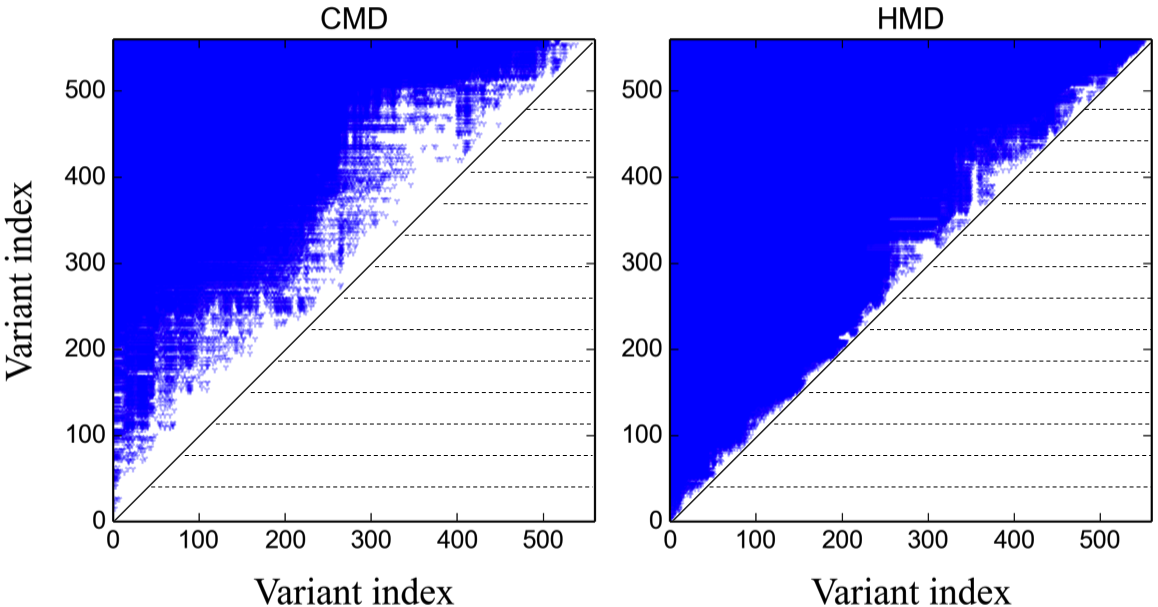
\includegraphics[width=\figSizeEightyFive]{ch06_patterns/figures/SimilarityEvaluation/StatisticalDiff.png}
	\end{center}
	\caption{Matrix indicating the statistical significance of the performance difference between every variant pair for the \acrshort{msds_iitm_cmd} and the \acrshort{msds_iitb_hmd}. Variant pairs where the difference in the performance is statistically significant are marked by dots.}
	\label{fig:patterns_statistical_significance_similarity_evaluation}
\end{figure}


The MAP scores and the details of parameter settings for the \acrshort{msds_iitb_hmd} dataset are shown in~\tabref{tab:melodic_similarity_results} (bottom half). Compared to the \acrshort{msds_iitm_cmd}, the best MAP score for the \acrshort{msds_iitb_hmd} is higher (0.55). Amongst the top ranked variants there is no consensus on the sampling rate of the melody representation. All the top ranked variants have the same parameter values except the sampling rate. This suggests that the sampling rates considered in this study have no significant effect on the melodic similarity for the \acrshort{msds_iitb_hmd}. This can be attributed to the fact that the recordings in the \acrshort{msds_iitb_hmd} are slow-medium tempo music pieces that do not have fast oscillatory melodic movements, as was the case with the \acrshort{msds_iitm_cmd}.  Furthermore, for the \acrshort{msds_iitb_hmd}, we observe that the variants using $N_{\mathrm{tonic}}$, $N_{\mathrm{tonicQ12}}$ or $N_{\mathrm{tonicQ24}}$ perform better than the ones using $N_{\mathrm{mean}}$, which is in contrast to the observation for the \acrshort{msds_iitm_cmd}. This is primarily because in Carnatic music in our datasets there are many cases where a pattern recurs in a different octave within the same recording, whereas, in Hindustani music, such cases are rare. In general, we see that the \gls{dtw}-based distance performs better than the euclidean distance, and the \gls{dtw} variant without a global constraint ($D_{\mathrm{DTW\_L1\_G90}}$ or $D_{\mathrm{DTW\_L0\_G90}}$) is preferred. This implies that the repeated instances of melodic patterns in IAM (specifically in Hindustani music) have large non linear timing variations.

To assess the statistical significance of the results we compare every possible pair of the variants ($^{560}C_{2}$ = 156520 comparisons). The results are shown in~\figref{fig:patterns_statistical_significance_similarity_evaluation}, where both the axes are the index of the variants in the ranked list. For every variant pair with index $i$ and $j$, we mark the pixel~($i$,$j$) if the difference is statistically significant. From~\figref{fig:patterns_statistical_significance_similarity_evaluation} we see that a majority of variant pairs have a statistically significant difference in the MAP scores. This indicates that the task of computing melodic similarity is sensitive to the choice of parameters and processing steps, and a small change in the choices made in a variant can lead to a significantly different MAP score. Furthermore, as the marked pixels are higher in number for the \acrshort{msds_iitb_hmd}, this sensitivity is even higher for the \acrshort{msds_iitb_hmd} compared to the \acrshort{msds_iitm_cmd}.


\begin{figure}
	\begin{center}
		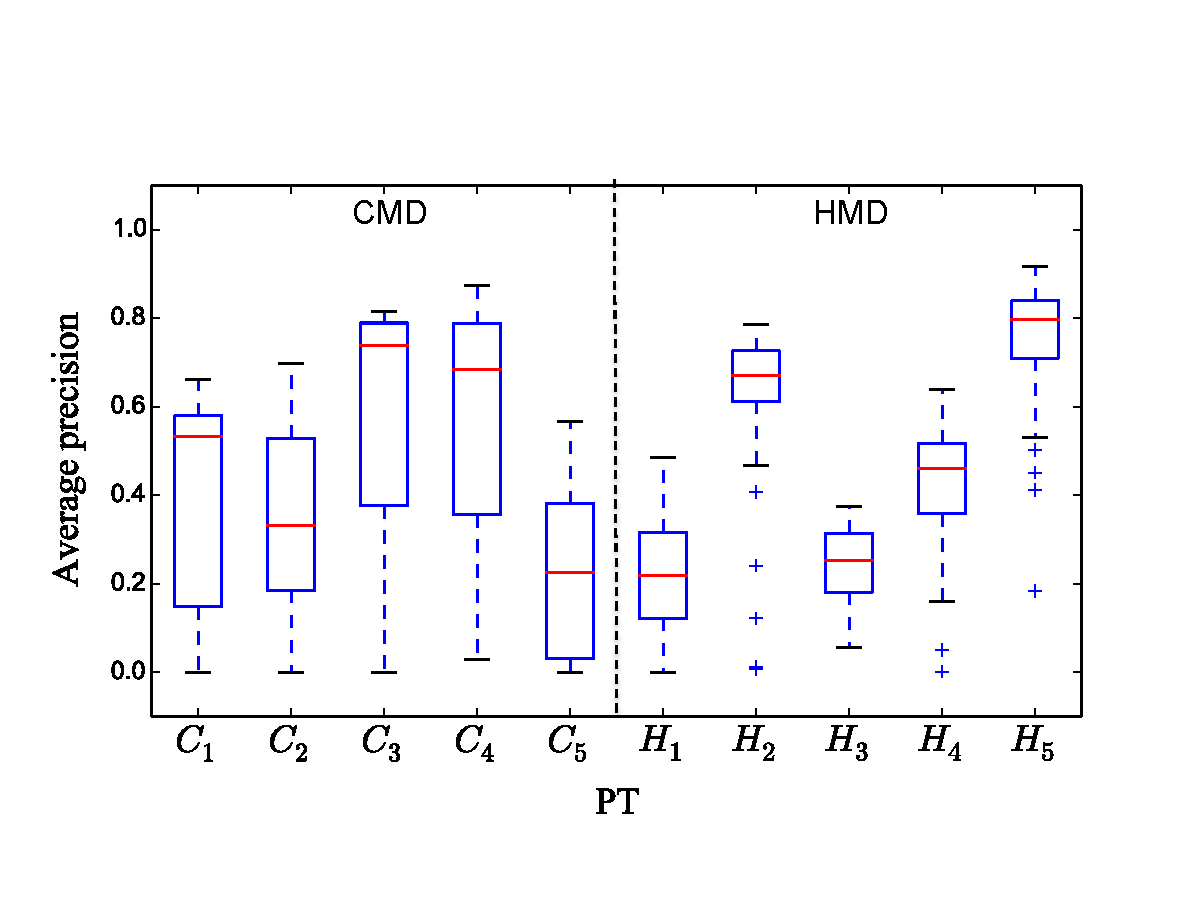
\includegraphics[width=\figSizeEightyFive]{ch06_patterns/figures/SimilarityEvaluation/CMD_HMD_CW_MAP.pdf}
	\end{center}
	\caption{Boxplot of the average precision values for each pattern type~(PT) in the \acrshort{msds_iitm_cmd} and the \acrshort{msds_iitb_hmd}.}
	\label{fig:patterns_similarity_evaluation_results_boxplot}
\end{figure}


To analyze the consistency in performance across pattern types, we present the boxplot of the average precision values for each pattern type in~\figref{fig:patterns_similarity_evaluation_results_boxplot}. For this, we consider only the top performing variant for each dataset. We see that the MAP scores vary considerably across pattern types for both the \acrshort{msds_iitm_cmd} and the \acrshort{msds_iitb_hmd}. Furthermore, we observe that the intra pattern type variance of the MAP scores is higher for the \acrshort{msds_iitm_cmd} as compared to the \acrshort{msds_iitb_hmd}. In addition, we observe that the pattern types $H_2$ and $H_5$ have a higher MAP value compared to other pattern types in the \acrshort{msds_iitb_hmd}. Interestingly, $H_2$ and $H_5$ are also the pattern types for which $L_{\mathrm{std}}$ is lower and $\#Occ$ is higher than others in the \acrshort{msds_iitb_hmd} (\tabref{tab:categorywise_details_melodic_similarity_dataset}). This correlation is not evident in the \acrshort{msds_iitm_cmd}, since $L_{\mathrm{std}}$ is small for all pattern types. 


\begin{table} 
	\begin{centering}
		\tabcolsep = 0.12cm
		\begin{tabular}{ c | c c c c c}
			\tabletop
			Dataset   	& 	MAP	&	Srate		&	Norm 	&	TScale 		&	Dist \\	
			\tablemid
			\multirow{3}{*}{\acrshort{msds_iitm_cmd}}   	
			& 	0.279 	&	$S_{67}$		&	$N_{\mathrm{mean}}$ 	&	$U_{\mathrm{on}}$		&	$D_{\mathrm{DTW\_L1\_G10}}$\\	
			& 	0.277 	&	$S_{67}$		&	$N_{\mathrm{tonicQ12}}$ 	&	$U_{\mathrm{on}}$		&	$D_{\mathrm{DTW\_L1\_G10}}$\\	
			& 	0.275	&	$S_{100}$		&	$N_{\mathrm{tonicQ12}}$ 	&	$U_{\mathrm{on}}$		&	$D_{\mathrm{DTW\_L1\_G10}}$\\	
\tablemid
			\multirow{3}{*}{\acrshort{msds_iitb_hmd}}   	
			& 	0.259	&	$S_{40}$		&	$N_{\mathrm{tonicQ12}}$ 	&	$U_{\mathrm{on}}$		&	$D_{\mathrm{DTW\_L1\_G90}}$\\	
			& 	0.259 	&	$S_{100}$		&	$N_{\mathrm{tonicQ12}}$ 	&	$U_{\mathrm{on}}$		&	$D_{\mathrm{DTW\_L1\_G90}}$\\	
			& 	0.259 	&	$S_{67}$		&	$N_{\mathrm{tonicQ12}}$ 	&	$U_{\mathrm{on}}$		&	$D_{\mathrm{DTW\_L1\_G90}}$\\	
			\tablebot		
		\end{tabular}
		\caption{MAP score and the details of parameter settings for the three best performing variants for the \acrshort{msds_iitm_cmd} and the \acrshort{msds_iitb_hmd} dataset. These results are corresponding to the experiment where target patterns' length is not read from the ground-truth annotations but is considered to be same as the query pattern length. Srate: sampling rate of the melody representation, Norm: normalization technique, TScale: uniform time-scaling and  Dist: distance measure.}
		\label{tab:melodic_similarity_results_var2}
\par \end{centering}		
\end{table}

So far we have considered segmented melodic patterns obtained using ground-truth annotations. For large audio archives such annotations are rarely available~(\secref{sec:patterns_melodic_pattern_discovery}). To simulate a retrieval scenario where the pattern boundaries are not known \textit{a priori}, we consider a simple extension to the experiment by assuming the target pattern length to be equal to the length of the query pattern. We evaluate all 560 variants of the method as done above on both the datasets under this experimental setup. In~\tabref{tab:melodic_similarity_results_var2} we show the MAP scores of the top performing variants for both the datasets \acrshort{msds_iitm_cmd} and \acrshort{msds_iitb_hmd}. We find that the MAP score for the best performing variant decreases from 0.41 to 0.28 and 0.55 to 0.26 for the \acrshort{msds_iitm_cmd} and the \acrshort{msds_iitb_hmd}, respectively. This indicates that the melodic similarity computation task becomes much more challenging in the absence of an accurate melodic segmentation method. For this experimental setup the trend in the sampling rate for Carnatic and Hindustani music remain the same as we saw in~\tabref{tab:melodic_similarity_results}, which is that a higher sampling rate is desired for representing melodic patterns in Carnatic music. In terms of the normalization we see that surprisingly $N_{\mathrm{tonicQ12}}$ is used by the top performing variants for both the datasets. Note that in other variants whose performance is not statistically significantly different from the ones reported in~\tabref{tab:melodic_similarity_results_var2}, $N_{\mathrm{mean}}$ and $N_{\mathrm{tonic}}$ normalization is also used for the \acrshort{msds_iitm_cmd} and the \acrshort{msds_iitm_cmd} dataset respectively. An interesting observation is that in this experimental setup uniform time-scaling is consistently used by all the top performing variants. This indicates that such a time-scaling operation is immensely advantages in the retrieval scenarios in \gls{iam} where the length of the target melodic patterns is taken to be the same as that of a query pattern. We also see that $D_{\mathrm{DTW\_L1\_G10}}$ and $D_{\mathrm{DTW\_L1\_G90}}$ are always used for the \acrshort{msds_iitm_cmd} and the \acrshort{msds_iitb_hmd} datasets, respectively, indicting that applying a local constraint in \gls{dtw} is critical for this experimental setup.

\TODO{If time permits it would be awesome to show accuracy as a function of different choices of parameters keeping others at an optimal value found in the grid search, This is similar to what we did for the latest raga recognition ISMIR paper.}

It is worth mentioning that compared to the existing studies~\cite{Ishwar2013, Ross2012b} we consider more number of pattern types and evaluate the performance of a variant using all annotated patterns as a query. Hence, the results presented are more likely to be generalizable and reliable. In the future we plan to include other aspects of melody such as loudness and timbre in the similarity computation and use a bigger dataset consisting of many more melodic patterns for evaluation.

\subsection{Summary}
\label{sec:patterns_melodic_similarity_summary}

We presented an evaluation of 560 different methodology variants for computing similarity of short-time melodic patterns in \gls{iam}. Our results indicate that the task of melodic similarity computation is very sensitive to the choice of parameters and processing steps. A higher sampling rate of the melody representation and mean normalization gives a better retrieval performance for Carnatic music. For Hindustani music, on the other hand, sampling rate has no significant affect on the performance and tonic normalization of the melody results in a better performance. In general, \gls{dtw}-based distance measure performs better than the Euclidean distance, and the usage of local constraint in \gls{dtw} enhances the performance. The \gls{dtw} variant without any global constraint is preferred (specially for Hindustani music), which suggests that there are large non-linear timing variations across repeated instances of the melodic pattern in \gls{iam}. We also see that accurate segmentation of melodic patterns has a big impact on the computation of melodic similarity.

\TODO{We have evaluated distance measure in supervised setup, we have not learned the distance measure or nuances from the data. THough learning parameters is also a way to learn from the data. But the bottle neck for now and which shuold be a future directino is that we need to learn specific nuances which matter, which might be dependent on the raga}

%################################################################################################################
%########################################### IMPROVING MELODIC SIMILARITY #######################################
%################################################################################################################


\section{Improving Melodic Similarity in Indian Art Music}
\label{sec:patterns_improving_melodic_similarity}

In \secref{sec:patterns_evaluation_of_similarity_measures} we performed a comparative evaluation of different system parameters and procedures typically involved in the computation of melodic similarity. Our objective was to study the influence of different parameters and procedures on melodic similarity, and to analyze how specific melodic  characteristics of Hindustani and Carantic music impact the optimal parameter setting. In this section we build upon our findings in \secref{sec:patterns_evaluation_of_similarity_measures} and present an approach that exploits specific melodic characteristics of Hindustani and Carnatic music to improve melodic similarity. 

Studies suggests that melodic similarity models may vary considerably depending on the type of music material (sheet music or polyphonic audio recordings)~\citep{Marsden2012, collins2014bridging, ghias1995query} and the music tradition~\citep{Juhasz2009a, Conklin2010a}. Results until now indicate that the important characteristics of several melody-dominant music traditions of the world such as Flamenco and \gls{iam} need dedicated research efforts to devise specific approaches for computing melodic similarity~\citep{Pikrakis2012, Rao2014}. With this spirit of devising culture specific approaches several methods for retrieving different types of melodic patterns have been proposed for \gls{iam} during the course of this dissertation~\citep{Ross2012b,Ross2012,ishwar2012motivic,Rao2014,Ishwar2013,Dutta2014}. 

\cite{Ross2012b} detect the occurrences of the title phrases of a composition within a concert recording of Hindustani music. The authors exploited the underlying rhythm structure to reduce the search space for detecting pattern occurrences. An extension of that approach~\citep{Ross2012} pruned the search space by employing a melodic landmark called \gls{nyas} \gls{svara} (Section XX). \cite{Rao2014} address the challenge of a large within-class variability in the occurrences of the characteristic phrases. They propose to use exemplar-based matching after vector quantization-based training to obtain multiple templates for a given phrase category. In addition, the authors propose to learn the optimal DTW constraints in a previous step for each phrase category in order to exploit the possible patterns in the duration variability. For Carnatic music, \cite{Ishwar2013} propose a two-stage approach for spotting the characteristic melodic phrases. The authors exploit specific melodic characteristics (saddle points) to reduce the target search space and use a distance measure based on rough longest common subsequence~\citep{lin2011music}. These approaches are important steps towards developing culturally informed and knowledge-driven information technologies to handle diversities in musics of the world. This is just a beginning and there is a large room for improvement in this area. As we just saw, a number of these approaches exploit specific melodic characteristics in \gls{iam} to prune the search space. However, most of them work on a specific form of music within Hindustani and Carnatic music and are hardly generalizable to even an entire music tradition. Moreover, the pruning power of these approaches and limitations are yet to be formally and comprehensively studied. Some of these approaches propose promising solutions to handle large within-class variability in melodic patterns, but these solutions are designed for supervised analysis of melodic patterns and are clearly not applicable to unsupervised analysis, which is one of our end goals in this dissertation.



\begin{figure}
	\begin{center}
		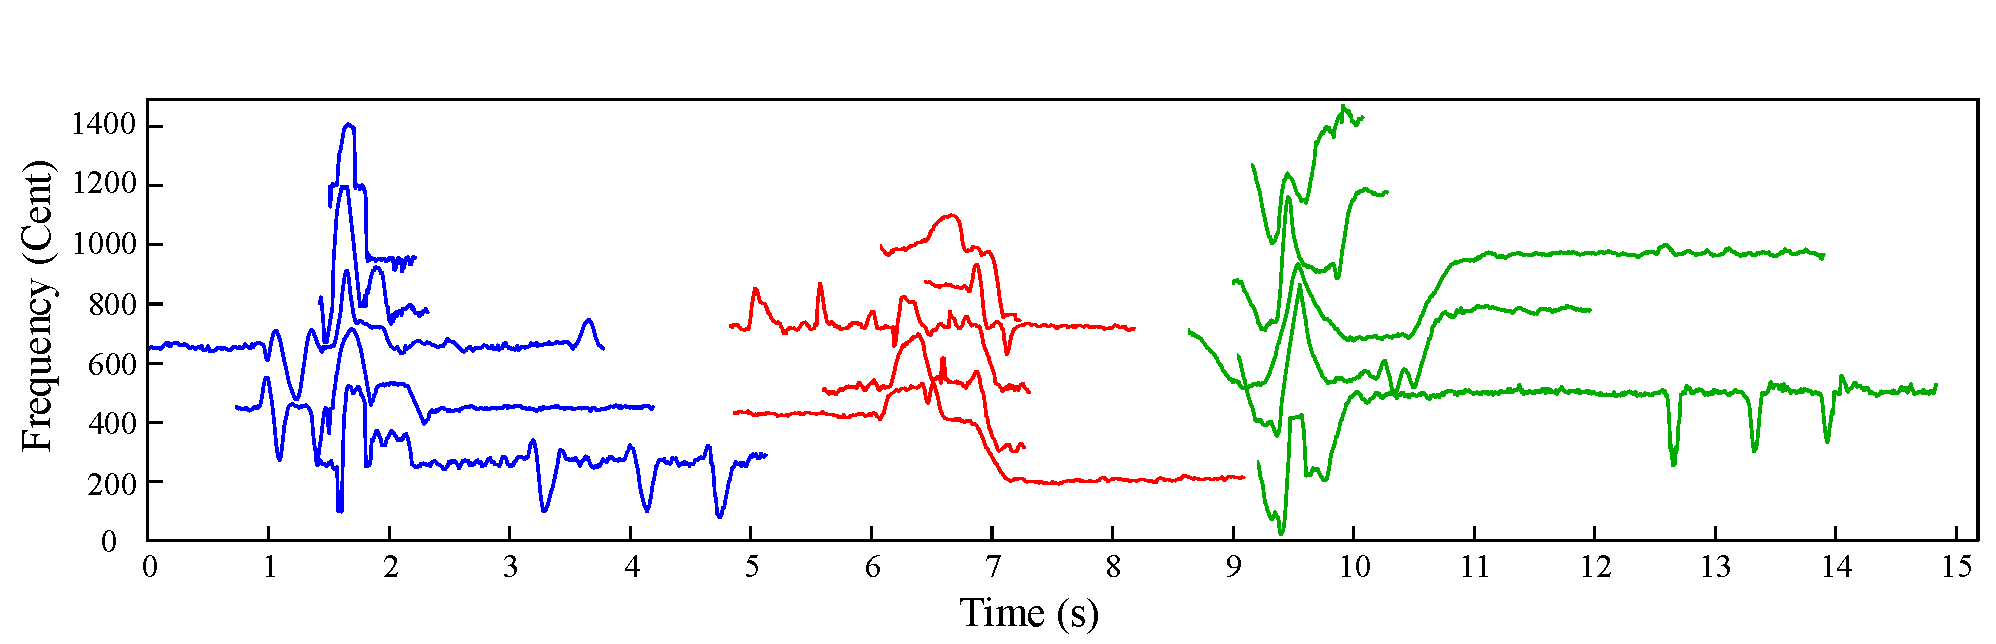
\includegraphics[width=\figSizeHundred]{ch06_patterns/figures/ImprovingSimilarity/phraseClassesExample.pdf}
	\end{center}
	\caption{Pitch contours of occurrences of three different characteristic melodic phrases in Hindustani music. Contours are frequency transposed and time shifted for a better visualization.\TODO{diff aspect ratio?}}
	\label{fig:phraseComplexityExample}
\end{figure}

It is worth revising the main challenges involved in computing melodic similarity for characteristic melodic phrases of \glspl{raga}. As already mentioned, the characteristic melodic phrases act as the basis for the artists to improvise, providing them with a medium to express creativity during a \gls{raga} rendition. Hence, the surface representation of these melodic phrases can vary a lot across their occurrences. This high degree of variability in terms of the duration of a phrase, non-linear time warpings and the added melodic ornaments together pose a big challenge for melodic similarity computation. In Figure~\ref{fig:phraseComplexityExample} we illustrate this variability by showing the pitch contours of the different occurrences of three characteristic melodic phrases of the \gls{raga} Alaiya Bilawal. We can clearly see that the duration of a phrase across its occurrences varies a lot and the steady melodic regions are highly varied in terms of the duration and the presence of melodic ornaments. Because of these and other factors, detecting the occurrences of characteristic melodic phrases becomes a challenging task. Ideally, the melodic similarity measure should be robust to a such high degree of melodic variations and, at the same time, it should be able to discriminate between different phrase categories and irrelevant melodic fragments (noise candidates).

In this section we present two approaches that utilize specific melodic characteristics in \gls{iam} to improve melodic similarity. We describe a melodic abstraction process based on a partial transcription of melodies to handle large timing variations across occurrences of melodic phrases. For Carnatic music we also present a complexity weighting scheme that accounts for the differences in the melodic complexities of the phrases, a crucial aspect for melodic similarity in this music tradition. The following sections are based on our work presented in~\cite{gulati_ISMIR_2015}.

\TODO{Highlight that we are incorporating and exploiting universal or transversal kind of characteristics. Specific nuances which are often raga specific and are very important for melodic similarity might be not possible since we do not have comprehensive annotated dataset.}


\subsection{Method}
\label{sec:patterns_improving_similarity_method}

Before we present our approach in detail we first discuss the motivation and rationale behind it. A close examination of the occurrences of the characteristic melodic phrases in our dataset reveals that there is a pattern in the non-linear timing variations, which is also reported in~\cite{Rao2014}. In~\figref{fig:phraseComplexityExample} we show a few occurrences of three such melodic phrases. In particular, we see that the transient regions of a melodic phrase tend to span nearly the same time duration across different occurrences, whereas the stationary regions vary a lot in terms of the duration. In~\figref{fig:flatCompressionExample} we further illustrate this by showing two occurrences of a melodic phrase ($P_{1a}$ and $P_{2a}$). The stationary \gls{svara} regions are highlighted. We clearly see that the duration variation is prominent in the highlighted regions. To handle such large non-linear timing variations typically a non-constrained \gls{dtw} distance measure is employed~(\secref{sec:patterns_melodic_similarity_results_discussions}). However, such a \gls{dtw} variant is also prone to noisy matches. Moreover, the absence of a band constraint renders it inefficient for computationally complex tasks such as pattern discovery~(\secref{sec:patterns_melodic_pattern_discovery}).

We put forward an approach that abstracts the melodic representation and reduces the extent of duration and pitch variations across the occurrences of a melodic phrase. Our approach is based on the partial transcription of the melodies.  As mentioned earlier, melodic transcription in \gls{iam} is a challenging task. The main challenges arise due to the presence of non-discrete pitch movements such as smooth glides and \glspl{gamaka}. However, since the duration variation exists mainly during the steady \gls{svara} regions, transcribing only the stable melodic regions might be sufficient. Once transcribed, we can then truncate the duration of these steady melodic regions and hence effectively reduce the amount of timing variations across the occurrences of a melodic phrase. Additionally, since the duration truncation also reduces the overall length of a pattern, the computational time for melodic similarity computation is also reduced substantially. Furthermore, this solution is independent of the distance measure used in the melodic similarity computation. Hence, it can be used even in the computationally complex tasks such as large scale pattern discovery, where the usage of distance lower bounds is imperative~(\secref{sec:patterns_melodic_pattern_discovery}).

\begin{figure}
	\begin{center}
		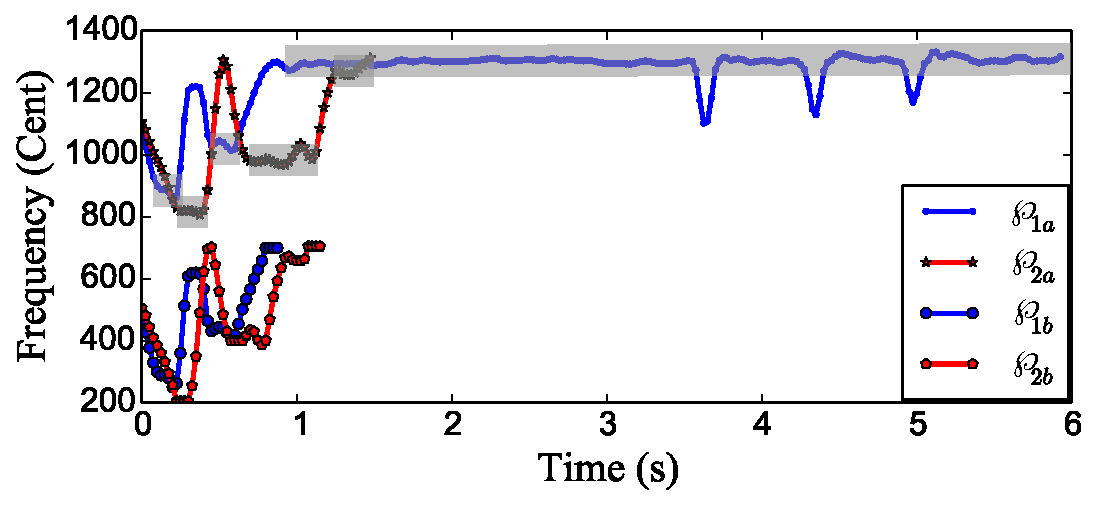
\includegraphics[width=\figSizeEightyFive]{ch06_patterns/figures/ImprovingSimilarity/Hindusani_flat_note_compression_example_reversed.pdf}
	\end{center}
	\caption{Original pitch contours ($P_{1a}$, $P_{2a}$) and duration truncated pitch contours ($P_{1b}$, $P_{2b}$) of two occurrences of a characteristic phrase of \gls{raga} Alhaiya Bilawal. The contours are transposed for a good visualization.}
	\label{fig:flatCompressionExample}
\end{figure}

\begin{figure}
	\begin{center}
		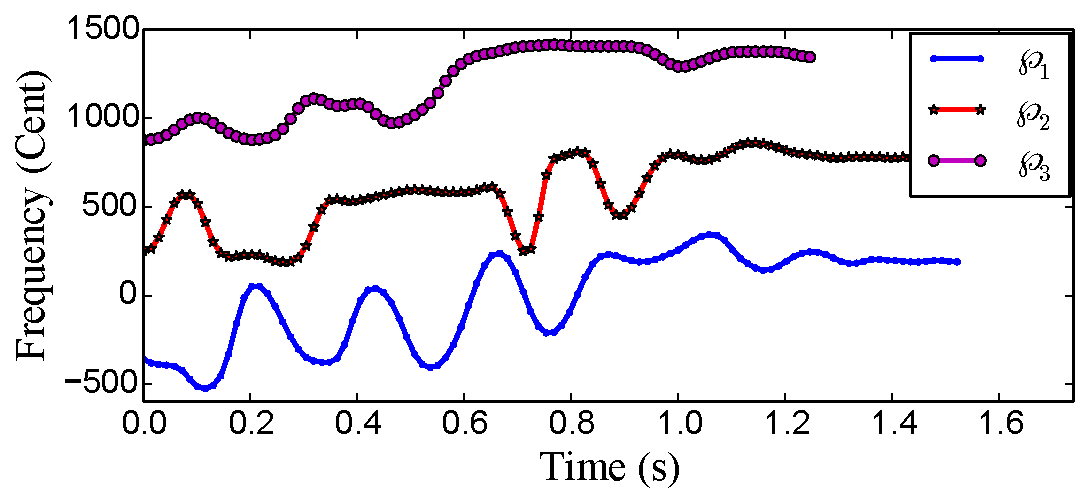
\includegraphics[width=\figSizeEightyFive]{ch06_patterns/figures/ImprovingSimilarity/CarnaticComplexityExample.pdf}
	\end{center}
	\caption{Pitch contours of three melodic phrases ($p_1$, $p_2$, $p_3$). $p_1$ and $p_2$ are the occurrences of the same characteristic phrase and both are musically dissimilar to $p_3$.} 
	\label{fig:carnaticComplexityExample}
\end{figure}

The rapid oscillatory pitch movements (\glspl{gamaka}) in Carnatic music bring up another set of challenges for the melodic similarity computation. Very often, two musically dissimilar melodic phrases obtain a high similarity score owing to a similar pitch contour at a macro level. However, they differ significantly at a micro level. In~\figref{fig:carnaticComplexityExample} we illustrate such a case where we show the pitch contours of three melodic phrases $P_1$, $P_2$ and $P_3$, where $P_1$ and $P_2$ are the occurrences of the same melodic phrase and both are musically dissimilar to $P_3$. Using the best performing variant of the similarity measure obtained in~\secref{sec:patterns_melodic_similarity_results_discussions} (\tabref{tab:melodic_similarity_results}) we obtain a higher similarity score between the pairs ($P_1$, $P_3$) and ($P_2$, $P_3$) compared to the score between the pair ($P_1$, $P_2$). This tendency of a high complexity time-series (higher degree of micro level variations) obtaining a high similarity score with another low complexity time-series is discussed in~\cite{batista2011complexity}. We follow their approach and apply a complexity weighting to account for the differences in the melodic complexities between phrases in the computation of melodic similarity. In the subsequent sections we present our proposed approach in detail. 


\subsubsection{Melody Estimation and post-processing}
\label{sec:patterns_improving_similarity_melody_estimation}

We represent melody of an audio signal by the pitch of the predominant melodic source. For predominant pitch estimation we follow exactly the same procedure and use the same parameter values as done in~\secref{sec:patterns_melodic_similarity_representation}, which is explained in detail in~\secref{sec:data_preprocessing_predominant_melody_estimation}. After estimating the predominant pitch we convert it from Hertz to Cent scale for the melody representation to be musically relevant~(\secref{sec:data_processing_cent_conversion}).

We proceed to post-process the pitch contours to remove the spurious pitch jumps lasting over a few frames as well as to smooth the pitch contours. We follow the procedure described in~\secref{sec:data_processing_pitch_smoothening} and use exactly the same set of parameter values. The pitch contours are finally down-sampled to 100\,Hz using the procedure described in~\secref{sec:data_processing_pitch_resampling}. This was found to be an optimal sampling rate for both Carnatic and Hindustani music in our earlier study that evaluated five different sampling rates~\secref{sec:patterns_melodic_similarity_results_discussions}. \TODO{Do we apply octave correction in here?, search for th documentation of how the pitch tracks are extracted}


\subsubsection{Transposition Invariance}
\label{sec:patterns_improving_similarity_transposition_invariance}

The base frequency chosen for a melody in \gls{iam} is the tonic pitch of the lead artist~(\secref{sec:data_preprocessing_tonic_identification}). Therefore, for a meaningful comparison of the melodic phrases across the recordings of different artists, a melody representation should be normalized by the tonic pitch of the lead artist. We perform this tonic normalization ($N_{tonic}$) by considering the tonic of the lead artist as the reference frequency during the Hertz to Cent conversion as shown in~\secref{sec:data_processing_cent_conversion}. The tonic pitch is automatically identified using a multi-pitch approach proposed by~\cite{salamon2012multipitch}. This approach performed the best in our comparative evaluation of seven different approaches~\secref{sec:pre_processing_tonic_identification_results}.

Tonic normalization does not account for the pitch of the octave transposed occurrences of a melodic phrase with-in a recording. In addition, estimated tonic pitch sometimes might be incorrect and a typical error is an offset of an octave or a fifth scale degree in some cases. To handle such cases, we propose a tetrachord normalization ($N_{tetra}$). For this we analyse the difference ($\Delta$) in the mean frequency values of the two tonic normalized melodic phrases ($p_1$, $p_2$). We offset the pitch values of the phrase $p_1$ by the frequency in the set $\lbrace$-\,1200, -\,700, -\,500, 0, 500, 700, 1200, 1700, 1900$\rbrace$ that is closest to $\Delta$ within a vicinity of 100\,cents. In addition to tetrachord normalization, we also experiment with mean normalization ($N_{mean}$), which was reported to improve the performance in the case of Carnatic music~(\secref{sec:patterns_melodic_similarity_results_discussions}). 


\subsubsection{Partial Transcription}
\label{sec:patterns_improving_similarity_partial_transcription}

We perform a partial melody transcription to automatically segment and identify the steady \gls{svara} regions in a melody. Note that even a partial transcription of the melodies is a non-trivial task, since we desire a segmentation that is robust to different melodic ornaments added to a \gls{svara} where the pitch deviation from the mean \gls{svara} frequency can be up to 200\,cents. In~\figref{fig:flatCompressionExample} we show such an example of a steady \gls{svara} region ($P_{1a}$ from 3-6\,s) where the pitch deviation from the mean \gls{svara} frequency is high due to added melodic ornaments. Ideally, the melodic region between 1 and 6\,s should be detected as a single \gls{svara} segment.

We segment the steady \gls{svara} regions using a method described in~\cite{gulati2014Landmark} (\secref{sec:pre_processing_nyas_segmentation}), which addresses the aforementioned challenges. A segmented \gls{svara} region is then assigned a frequency value corresponding to the peak in an aggregated pitch histogram closest to the mean \gls{svara} frequency. The pitch histogram is constructed for the entire recording and smoothened using a Gaussian window with a variance of 15\,cents. As peaks of the normalized pitch histogram, we select all the local maximas where at least one peak-to-valley ratio is greater than 0.01. A detailed description of this method is provided in~\secref{sec:pre_processing_nyas_segmentation}.
 
\subsubsection{Svar Duration Truncation}
\label{sec:patterns_improving_similarity_svara_duration_trucation}

After segmenting the steady \gls{svara} regions in the melodies we proceed to truncate the duration of these regions. We hypothesize that, beyond a certain value $\delta$, the duration of these steady \gls{svara} regions do not change the identity of a melodic phrase (i.e.~the phrase category). We experiment with 7 different truncation durations $\delta = \lbrace$ 0.1\,s, 0.3\,s, 0.5\,s, 0.75\,s, 1\,s, 1.5\,s, 2\,s$\rbrace$ and select the one that results in the best performance. In~\figref{fig:flatCompressionExample}
we show an example of the occurrences of a melodic phrase both before ($P_{1a}$, $P_{2a}$) and after ($P_{1b}$, $P_{2b}$) the \gls{svara} duration truncation using $\delta = 0.1$\,s. This example clearly illustrates that the occurrences of a melodic phrase after duration truncation exhibit lower degree of non-linear timing variations. We denote this method by $M_{DT}$.

\subsubsection{Similarity Computation}
\label{sec:patterns_improving_similarity_similarity_computation}

To measure the similarity between two melodic fragments we consider a \gls{dtw}-based approach. Since the phrase segmentation is known beforehand, we use a whole sequence matching \gls{dtw} variant. We consider the best performing \gls{dtw} variant and the related parameter values for each music tradition as reported in~\secref{sec:patterns_melodic_similarity_results_discussions}. These variants were chosen based on an exhaustive grid search across all possible combinations and hence can be considered as optimal for this dataset. For Carnatic music we use a \gls{dtw} step size condition $\lbrace(2,1), (1,1), (1,2)\rbrace$  and for Hindustani music a step size condition $\lbrace(1,0), (1,1), (0,1)\rbrace$.  We use Sakoe-Chiba global band constraint~\cite{Sakoe78TASLP} with the width of the band as $\pm10$\% of the phrase length. Before computing the \gls{dtw} distance we uniformly time-scale the two melodic fragments to the same length, which is the maximum of the lengths of the phrases. Notice that even though in~\secref{sec:patterns_melodic_similarity_results_discussions} we found that a globally unconstrained \gls{dtw} variant ($D_{\mathrm{DTW\_L0\_G90}}$) is an optimal choice for computing melodic similarity in Hindustani music, we restrict ourselves to a band-width of 10\% in this study. The main reason is because an unconstrained \gls{dtw} variant due to its computational complexity is not suitable for a large scale pattern discovery task~(\secref{sec:patterns_melodic_pattern_discovery}). Since one the main objectives of studying melodic similarity within a supervised setup in this work is to be finally able to apply the findings in an unsupervised analysis, we now restrict to choices that are also available and feasible in an unsupervised analysis. \TODO{rephrase the last part}


\subsubsection{Complexity Weighting}
\label{sec:patterns_improving_similarity_complexity_invariance_weighting}

The complexity weighting that we apply here to overcome the shortcoming of the distance measure in distinguishing two time series with different complexities is discussed in~\cite{batista2011complexity}. We apply a complexity weighting ($\alpha$) to the \gls{dtw}-based distance ($D_{DTW}$) in order to compute the final similarity score $D_{f}=\alpha D_{DTW}$. We compute $\alpha$ as:


\begin{equation}
\begin{gathered}
\alpha = \frac{\max(C_i,C_j)}{\min(C_i, C_j)} \\
%C_i = \sqrt[2]{\sum_{i=1}^{N-1} (p_{i}-p_{i+1})^2}\\
\end{gathered}
\label{eq:complexity_weighing}
\end{equation}

\begin{equation}
\begin{gathered}
%\alpha = \frac{\max(C_i,C_j)}{\min(C_i, C_j)} \\
C_i = \sqrt[2]{\sum_{i=1}^{N-1} (p_{i}-p_{i+1})^2}\\
\end{gathered}
\label{eq:complexity_estimate_batista}
\end{equation}

\noindent where, $C_i$ is the complexity estimate of a melodic phrase of length $N$ samples and $p_i$ is the pitch value of the $i^{\mathrm{th}}$ sample. We explore two variants of this complexity estimate. One of these variants is already proposed in~\cite{batista2011complexity} and is described in equation~\ref{eq:complexity_estimate_batista2}. We denote this method variant by $M_{CW1}$. We propose another variant that utilizes melodic characteristics of Carnatic music. This variant takes the number of saddle points in the melodic phrase as the complexity estimate~\citep{Ishwar2013}. This method variant is denoted by $M_{CW2}$. As saddle points we consider all the local minimas and the local maximas in the pitch contour which have at least one minima to maxima distance of half a semitone. Since such melodic characteristics are predominantly present in Carnatic music, the complexity weighting is not applicable for computing melodic similarity in Hindustani music.


\subsection{Evaluation}
\label{sec:patterns_improving_similarity_evaluation}

\subsubsection{Dataset and Annotations}
\label{sec:patterns_improving_similarity_dataset_and_annotations}

For evaluation we use the same music collection as used in~\secref{sec:patterns_evaluation_of_similarity_measures}, which is described in~\secref{sec:corpus_melodic_similarity_dataset}. This collection enables a better comparison of the results with other studies since it has been used in several other studies for a similar task~\citep{Rao2014,Ross2012b}. However, we found a number of issues in the annotations of the melodic phrases, which we corrected and also extended the dataset by adding 25\% more number of melodic phrase annotations as explained in~\secref{sec:corpus_melodic_similarity_dataset}. We denote this new dataset by \acrshort{msds_cm} and the comprising Carnatic and Hindustani sub-datasets by \acrshort{msds_cm_cmd} and \acrshort{msds_cm_hmd}, respectively. Similar to the way we perform evaluations in~\secref{sec:patterns_evaluation_of_similarity_measures}, we evaluate our approach separately on both Carnatic and Hindustani datasets. In~\tabref{tab:melodic_similarity_dataset_details} we summarize the relevant details of the dataset in terms of the number of artists, \glspl{raga}, audio recordings and total duration. In~\tabref{tab:categorywise_details_revised_melodic_similarity_dataset} we summarize the details of the annotated phrases in terms of their number of instances and basic statistics of the length of the phrases.


\subsubsection{Setup, Measures and Statistical Significance}
\label{sec:patterns_improving_similarity_experimental_setup}

The experimental setup and evaluation measures used in this study are exactly the same as used for the comparative evaluation described in~\secref{sec:patterns_evaluation_of_similarity_measures}. We consider each annotated melodic phrase as a query and perform a search across all the annotated phrases in the dataset (referred to as target search space). In addition to the annotated phrases, we add randomly sampled melodic segments (referred to as noise candidates) in the target space to simulate a real world scenario. We generate the starting time stamps of the noise candidates by randomly sampling a uniform distribution. The length of the noise candidates are generated by sampling the distribution of the duration values of the annotated phrases. The number of noise candidates added are 100 times the number of total annotations in the entire music collection. For every query we consider the top 1000 nearest neighbours in the search results ordered by the similarity value. A retrieved melodic phrase is considered as a true hit only if it belongs to the same phrase category as the query. As a baseline in this study we consider the same method as described in this section but without applying the \gls{svara} duration truncation and complexity weighting procedure. We denote this baseline method by $M_{B}$.

To assess the performance of our approach and the baseline method we use mean average precision (MAP), a common measure in information retrieval~\citep{manning2008introduction}. To assess if the difference in the performance of any two methods is statistically significant we use the Wilcoxon signed rank-test~\citep{wilcoxon1945individual} with $p < 0.01$. To compensate for multiple comparisons, we apply the Holm-Bonferroni met-hod~\citep{holm1979simple}.


\subsection{Results and Discussion}
\label{sec:patterns_improving_similarity_results_and_discussion}

\TODO{if time permits, first report the accuracy of best variants of prev study on new dataset an then with post processing, and then with new method?, also the chosen config in the current study, it should be shown how that is behaving in previous study. Also should we also present var2 of our approach, i.e. with unknown segment lengths?}
\TODO{If time permits also experiment with NCR1, 10, 100, 1000 for the best config. That way we can know what is the affect of NCR!!}

In~\tabref{tab:patterns_improving_similarity_map_scores} we summarize the MAP scores and the standard deviation of the average precision values obtained using the baseline method ($M_{B}$), the method that uses duration truncation ($M_{DT}$) and the ones using the complexity weighting ($M_{CW1}$, $M_{CW2}$), for both the \acrshort{msds_cm_cmd} and the \acrshort{msds_cm_hmd}. Note that $M_{CW1}$ and $M_{CW2}$ are only applicable to the \acrshort{msds_cm_cmd} (\secref{sec:patterns_improving_similarity_complexity_invariance_weighting}).


\begin{table} 
	\begin{centering}
	\tabcolsep = 0.15cm
	\renewcommand{\arraystretch}{1.5}
	\begin{tabular}{ c | c  c  c  c }
\tabletop
		\multicolumn{5}{c }{\acrshort{msds_cm_hmd}}\\
\tablemid
		Norm &	$M_{B}$ & $M_{DT}$ &  $M_{CW1}$ & $M_{CW2}$\\
\tablemid		
		$N_{tonic}$	& {\bf 0.45 (0.25)}	&	{\bf 0.52 (0.24)} 	& - &-\\ 
		$N_{mean}$	& 0.25 (0.20)		&	0.31 (0.23) 		& - &-\\  	
		$N_{tetra}$	& 0.40 (0.23)		&	0.47 (0.23) 		& - &-\\  	
		
		%& $E_2$ & xxx	& 0.25	&	0.27 & - \\   
\tablebot
		\multicolumn{5}{c }{\acrshort{msds_cm_cmd}}\\
\tablemid
		Norm &	$M_{B}$ & $M_{DT}$ &  $M_{CW1}$ & $M_{CW2}$\\
		\hline
		$N_{tonic}$	&  0.39 (0.29)	&	0.42 (0.29) & 0.41 (0.28)&0.41 (0.29) \\ 
		$N_{mean}$	&  0.39 (0.26)	&	0.45 (0.28) & 0.43 (0.27)&0.45 (0.27) \\  	
		$N_{tetra}$	&  {\bf 0.45 (0.26)}	&	{\bf 0.50 (0.27)} & {\bf 0.49 (0.28)} &{\bf 0.51 (0.27)} \\  	
\tablebot	
		
	\end{tabular}
	\caption{MAP scores for the two datasets \acrshort{msds_cm_hmd} and \acrshort{msds_cm_cmd} for the four method variants $M_{B}$, $M_{DT}$, $M_{CW1}$ and $M_{CW2}$ and for different normalization techniques. Standard deviation of average precision is reported within round brackets.}
	\label{tab:patterns_improving_similarity_map_scores}
\par \end{centering}	
\end{table}


We first analyse the results for the \acrshort{msds_cm_hmd} dataset. From~\tabref{tab:patterns_improving_similarity_map_scores} (upper half), we see that the proposed method variant that applies a duration truncation performs better than the baseline method for all the normalization techniques. Moreover, this difference is found to be statistically significant in each case. The results  for the \acrshort{msds_cm_hmd} in this table correspond to $\delta=$500\,ms, for which we obtain the highest accuracy compared to the other $\delta$ values as shown in~\figref{fig:map_per_duration_truncation}. Furthermore, we see that $N_{tonic}$ results in the best accuracy for the \acrshort{msds_cm_hmd} for all the method variants and the difference is found to be statistically significant in each case. From~\tabref{tab:patterns_improving_similarity_map_scores} we notice a high standard deviation of the average precision values. This is because some occurrences of melodic phrases possess a large amount of melodic variation (acting as outliers), and therefore, the average precision value of the retrieved results using them as a query is much smaller compared to the other occurrences. In~\figref{fig:hinudstaniPerCategoryPerformance} we show a boxplot of average precision values for each phrase category and for both $M_B$ and $M_{DT}$ to get a better understanding of the results. We observe that with an exception of the phrase category $H_2$, $M_{DT}$ consistently performs better than $M_B$ for all the other phrase categories. A close examination of this exception reveals that the error often is in the segmentation of the steady \gls{svara} regions of the melodic phrases corresponding to $H_2$. This can be attributed to a specific subtle melodic movement in $H_2$ that is confused by the segmentation method as a melodic ornament instead of a \gls{svara} transition, leading to a segmentation error. \TODO{If time permits show an image of this pattern and the subtle movement!! if you plot images for all the patterns in the dataset refer to that}


\begin{figure}
	\begin{center}
		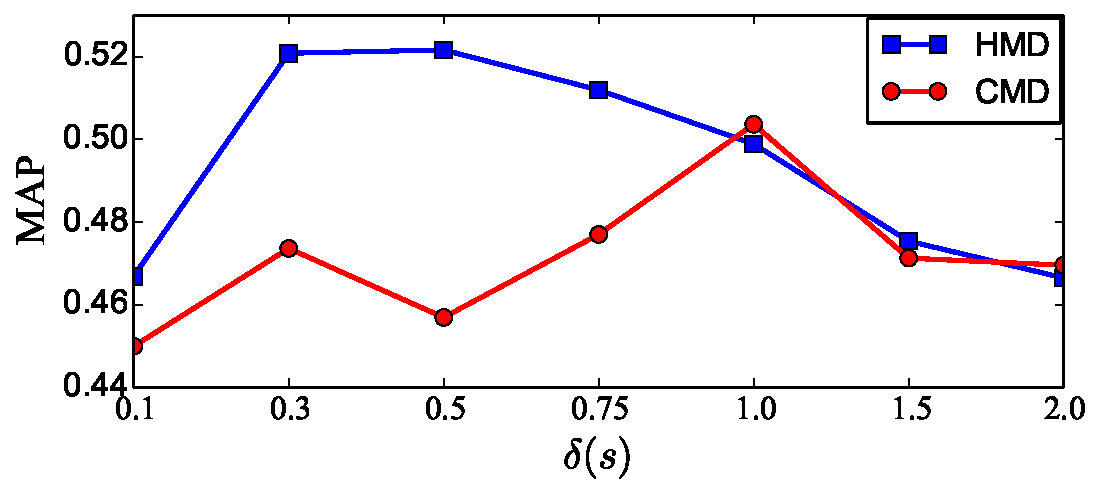
\includegraphics[width=\figSizeEightyFive]{ch06_patterns/figures/ImprovingSimilarity/MAP_per_Duration_Truncation.pdf}
	\end{center}
	\caption{MAP scores for different duration truncation values ($\delta$) for the \acrshort{msds_cm_hmd} and the \acrshort{msds_cm_cmd}.} 
	\label{fig:map_per_duration_truncation}
\end{figure}

\begin{figure}
	\begin{center}
		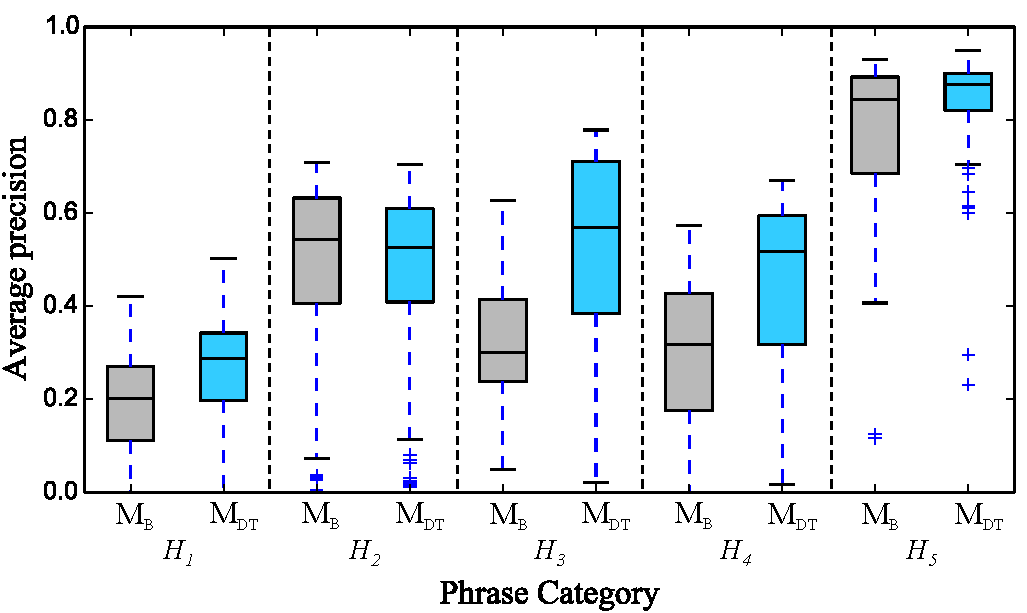
\includegraphics[width=\figSizeEightyFive]{ch06_patterns/figures/ImprovingSimilarity/HindustaniPerCategoryPerformance_BOXPLOT.pdf}
	\end{center}
	\caption{Boxplot of average precision values obtained using $M_{B}$ and $M_{DT}$ for each melodic phrase category for the \acrshort{msds_cm_hmd}. These values correspond to $N_{tonic}$.} 
	\label{fig:hinudstaniPerCategoryPerformance}
\end{figure}


We now analyse the results for the \acrshort{msds_cm_cmd} dataset. From~\tabref{tab:patterns_improving_similarity_map_scores} (lower half), we see that using the method variants $M_{DT}$, $M_{CW1}$ and $M_{CW2}$ we obtain reasonably higher MAP scores compared to the baseline method $M_{B}$ and the difference is found to be statistically significant for each method variant across all normalization techniques. This MAP score for $M_{DT}$ corresponds to $\delta=$1\,s, which is considerably higher than the MAP scores for other $\delta$ values as shown in~\figref{fig:map_per_duration_truncation}. We also see that $M_{CW2}$ performs slightly better than $M_{CW1}$ and the difference is found to be statistically significant only in the case of $N_{tetra}$. We do not find any statistically significant difference in the performance of methods $M_{DT}$ and $M_{CW2}$. Unlike in the case of the \acrshort{msds_cm_hmd} dataset, for the \acrshort{msds_cm_cmd} dataset $N_{tetra}$ results in the best performance with a statistically significant difference compared to the other normalization techniques across all method variants. We now analyse the average precision values for every phrase category for $M_B$, $M_{DT}$ and $M_{CW2}$. Since $M_{CW2}$ performs slightly better than $M_{CW1}$ we only consider $M_{CW2}$ for this analysis. In~\figref{fig:carnaticPerCategoryPerformance} we see that $M_{DT}$ performs better than $M_B$ for all phrase categories.  We also observe that $M_{CW2}$ consistently performs better than $M_{B}$ with the sole exception of $C_2$. This exception occurs because $M_{CW2}$ presumes a consistency in terms of the number of saddle points across the occurrences of a melodic phrase, which does not hold true for $C_2$. This is because phrases corresponding to $C_2$ are rendered very fast and the subtle pitch movements are not the characteristic aspect of such melodic phrases. Hence, the artists often take the liberty of changing the number of saddle points. 

\begin{figure}
	\begin{center}
		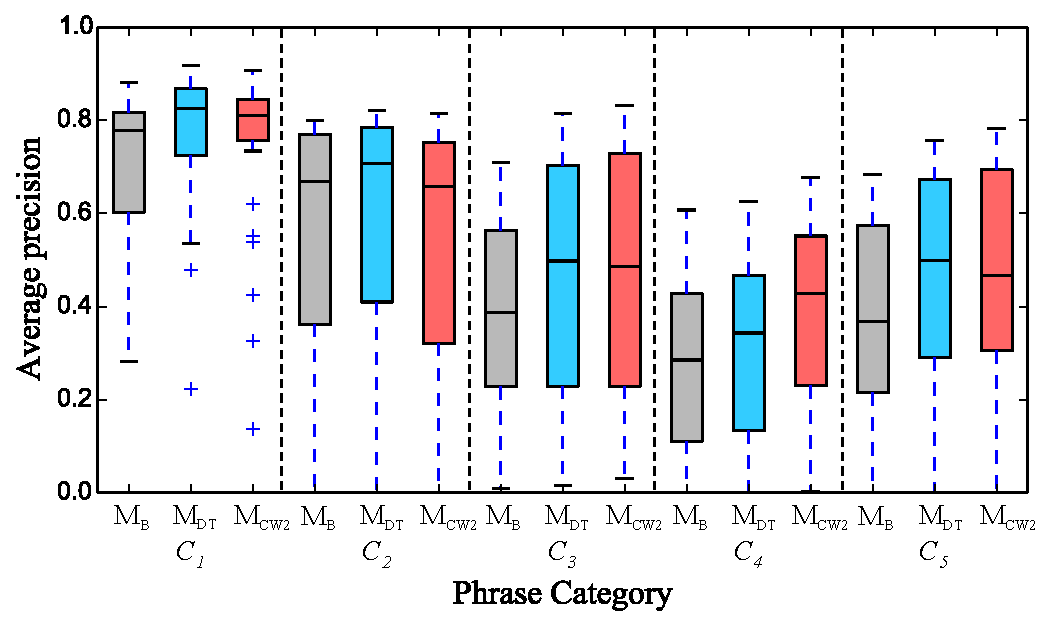
\includegraphics[width=\figSizeEightyFive]{ch06_patterns/figures/ImprovingSimilarity/CarnaticPerCategoryPerformance_BOXPLOT.pdf}
	\end{center}
	\caption{Boxplot of average precision values obtained using methods $M_{B}$, $M_{DT}$ and $M_{CW}$ for each melodic phrase category for the \acrshort{msds_cm_cmd}. These values correspond to $N_{tetra}$.}
	\label{fig:carnaticPerCategoryPerformance}
\end{figure}


Overall we see that duration truncation of steady melodic regions improves the performance in both \acrshort{msds_cm_hmd} and \acrshort{msds_cm_cmd} datasets. This reinforces our hypothesis that elongation of steady \gls{svara} regions in the melodies of \gls{iam} in the context of the characteristic melodic phrase does not change the musical identity of the phrase. This correlates with the concept of \gls{nyas} \gls{svara} (\secref{sec:backgroung_nyas_description}), where the artist has the flexibility to stay and elongate a single \gls{svara}. A similar observation was reported in~\cite{Rao2014}, where the authors proposed to learn the optimal global \gls{dtw} constraints a priori for each pattern category. However, as they report, their proposed solution could not improve the performance. Further comparing the results for the \acrshort{msds_cm_hmd} and \acrshort{msds_cm_cmd} datasets we notice that $N_{tonic}$ results in the best performance for the \acrshort{msds_cm_hmd} and $N_{tetra}$ for the \acrshort{msds_cm_cmd}. This can be attributed to the fact that the number of the pitch-transposed occurrences of a melodic phrase is significantly higher in the \acrshort{msds_cm_cmd} compared to the \acrshort{msds_cm_hmd} (\secref{sec:patterns_melodic_similarity_results_discussions}). Also, since the non-linear timing variability in the \acrshort{msds_cm_hmd} is very high, any normalization ($N_{mean}$ or $N_{tetra}$) that involves a decision based on the mean frequency of the phrase is more likely to fail.


\subsection{Summary}
\label{sec:patterns_improving_similarity_summary}

In this section we highlighted the major challenges involved in this task and focused on two specific issues that arise due to large non-linear timing variations and rapid melodic movements. We described simple and easy to implement solutions based on partial transcription and complexity weighting to address these challenges. We showed that duration truncation of the steady \gls{svara} regions in the melodic phrases results in a statistically significant improvement in the computation of melodic similarity. Furthermore, we showed that complexity weighting improves the melodic similarity in Carnatic music. This suggests that the extent and the number of saddle points is an important characteristic of a melodic phrase and is crucial to melodic similarity in Carnatic music.  In the future, we plan to improve the method used for segmenting the steady \gls{svara} regions so that it can differentiate melodic ornaments from subtle \gls{svara} transitions. In addition, we see a vast scope in further refining the complexity estimate of a melodic phrase to improve the complexity weighting. It would also be worthwhile to explore the applicability of this approach to music traditions such as Flamenco, Beijing opera and Turkish Makam music.

\TODO{ you can consider adding a section on limitations of the string matching basd similarity measures in the context of Indian art music. Give examples in situations which need specifric nuances in melodies to weigh more and which is completely not considered in our similarity measure. Say this as the future direction. Probably a model based method is what is needed and not string based matching. Read PhD doc that I have been writing to get more points on this.}


%################################################################################################################
%########################################### Melodic Pattern Discovery ##########################################
%################################################################################################################


\section{Melodic Pattern Discovery in Sizable Audio Collections}
\label{sec:patterns_melodic_pattern_discovery}

The task of melodic pattern discovery aims to mine repeating patterns in a time-series representation of melodies by following an unsupervised methodology. As mentioned before in \secref{sec:patterns_introduction}, extracting melodic patterns and detecting their different occurrences in audio music collections is crucial for melodic analyses of \gls{iam}. The discovered melodic patterns can be utilized in a number of other computational tasks and applications such as automatic \gls{raga} recognition, studying similarities between artists and different schools of music, meaningful music recommendations and developing pedagogical tools.

In \secref{sec:patterns_evaluation_of_similarity_measures} and \secref{sec:patterns_improving_melodic_similarity} we studied different approaches and their variants for computing similarities between short melodic fragments. Given instances of different melodic patterns by an domain expert, these approaches can be used to detect occurrences of such example patterns in audio music collections of \gls{iam}. However, as the size of the evaluation datasets \acrshort{msds_cm_hmd} and \acrshort{msds_cm_cmd} reflects, obtaining such example patterns is a cumbersome task. Moreover, there are several other challenges involved in compiling a comprehensive collection of all repeating patterns in a large audio collection of \gls{iam} (\secref{sec:patterns_introduction}). We therefore follow an unsupervised approach for extracting melodic patterns in audio music collections, and do not require any example melodic patterns. 

\TODO{write a better sota after reading more!}
In \gls{mir}, several approaches have been proposed for extracting different kinds of repeating structures, including long duration repetitions such as themes, choruses and sections~\cite{paulus2010state}, and short duration repetitions such as motifs and riffs~\cite{Janssen2013}. While there exists a number of approaches for motivic discovery in sheet music~\cite{Lartillot2005}, there are fewer approaches that work on audio music recordings~\cite{dannenberg2003pattern}. This can be attributed to the audio-symbolic gap \cite{collins2014bridging}, which can be bridged by a reliable automatic transcription system to abstract the audio music content into musically meaningful discrete symbols. There exists a wide scope for developing methodologies for the discovery and analysis of short duration melodic patterns (or motifs) in large audio music collections. In the case of audio music recordings, approaches for motif discovery can benefit from the literature in the domain of time series analysis such as time series representation~\cite{Lin2003}, core pattern discovery methods~\cite{Mueen2009}, and search and indexing techniques~\cite{Rakthanmanon2013}.

In recent years, many approaches have been proposed for this task, most of them of a supervised nature.  Ross~et~al.~\cite{Ross2012b} detect title phrases of a composition within a concert of Hindustani music. The authors use annotated rhythm cycle boundaries for pattern segmentation. Ishwar~et~al.~\cite{Ishwar2013} propose a two-stage approach and a sparse melody representation for spotting characteristic melodic patterns of a \gls{raga}. Rao~et~al.~\cite{Rao2014} classify melodic motives in IAM by using exemplar-based matching and propose an approach to learn DTW global constraints for computing melodic similarity. Many of these approaches either use semi-supervised pitch estimation, manually segmented pattern boundaries, a dataset comprising few recordings, or analyze only a limited number of characteristic phrases. Thus, scalability of such approaches is questionable and over-fitting of the approach to a specific dataset is probable. \TODO{see if something is usable otherwise delete}.


\TODO{do we write the ending statement before describing the method? look at the paper for some content!!}


\subsection{Method}
\label{sec:patterns_discovery_method}

\begin{figure}
	\begin{center}
		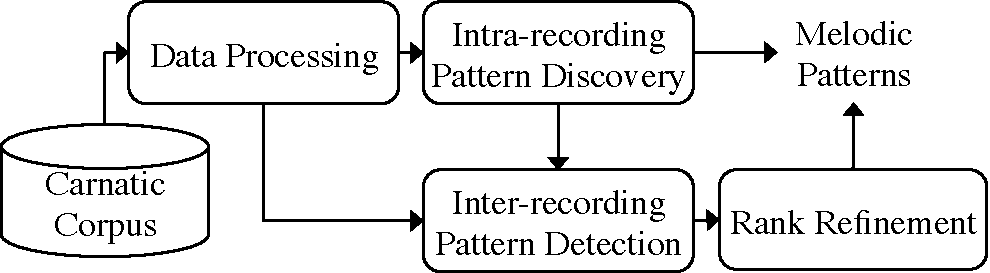
\includegraphics[width=\figSizeEightyFive]{ch06_patterns/figures/discovery/blockDiagram_Overall.pdf}
	\end{center}
	\caption{Block diagram of the proposed approach for melodic pattern discovery in large audio collections of \gls{iam}}
	\label{fig:pattern_discovery_overall_block_diagram}
\end{figure}

Our approach for pattern discovery in audio music collections consists of four main blocks as shown in~\figref{fig:pattern_discovery_overall_block_diagram}. The data processing block (\secref{sec:pattern_discover_preprocessing}) generates pitch subsequences from every audio recording in the music collection. The intra-recording pattern discovery block (\secref{sec:intraRecordingPatternDiscovery}) performs an exact pattern discovery by detecting the closest subsequence pairs within an audio recording (referred to as seed patterns). The inter-recording pattern detection block (\secref{sec:inter_recording_pattern_search}) considers each seed pattern as a query and searches for its occurrences in the entire music collection. The rank refinement block (\secref{sec:rankRefinement}) reorders a ranked list of search results by recomputing melodic similarity using a more sophisticated similarity measure. The following description is based on our work presented in~\cite{gulati_SITIS_2014}.

We choose to perform first an intra-recording pattern discovery because several melodic patterns are repeated within a music piece of Carnatic music. Moreover, the scalability of the computational approaches considered here for discovering patterns at the level of the entire music collection is questionable. To confirm this hypothesis, we conducted an experiment using a state-of-the-art algorithm for time series motif discovery~\citep{Mueen2009}, with a trivial modification to extract the top K motifs. Using just 16\,hours of audio data (amounting to around 20\,million pitch samples), the algorithm could discover only 40~melodic patterns in 24\,hours using Euclidean distance. Besides pattern pairs being from the same recording, only a few of the obtained pattern pairs were melodically similar and meaningful. This is expected as we found in \secref{sec:patterns_melodic_similarity_results_discussions} that Euclidean distance is not appropriate for handling large-non linear timing variations present across occurrences of melodic patterns. In order to scale the tasks of pattern discovery for hundreds of hours of audio data using a computationally complex \gls{dtw}-based distance measure we choose to first perform pattern discovery within an audio recording.

Before we proceed to describe our method it should be noted that during the course of this dissertation several processing blocks and system parameters presented in the subsequent sections have evolved. The methodology presented in this section is based on our work reported in~\cite{gulati_SITIS_2014}. However, after that study, based on our findings in ~\cite{gulati_ICASSP2015} and in~\cite{gulati_ICASSP2015} we have modified the procedure followed in several processing blocks and system parameters. In order to facilitate reproducibility of our experiments and research outcomes, along with the original description of the method~\citep{gulati_SITIS_2014} we also present the modifications done for the new (the most recent) variant of the method. Wherever applicable the modifications are presented during the description of the processing block. Since the evaluation methodology we followed involve cumbersome listening tests, the results presented in this section are only corresponding to the initial variant of the method presented in~\cite{gulati_SITIS_2014}.


\subsubsection{Pre-processing}
\label{sec:pattern_discover_preprocessing}

\begin{figure}
	\begin{center}
		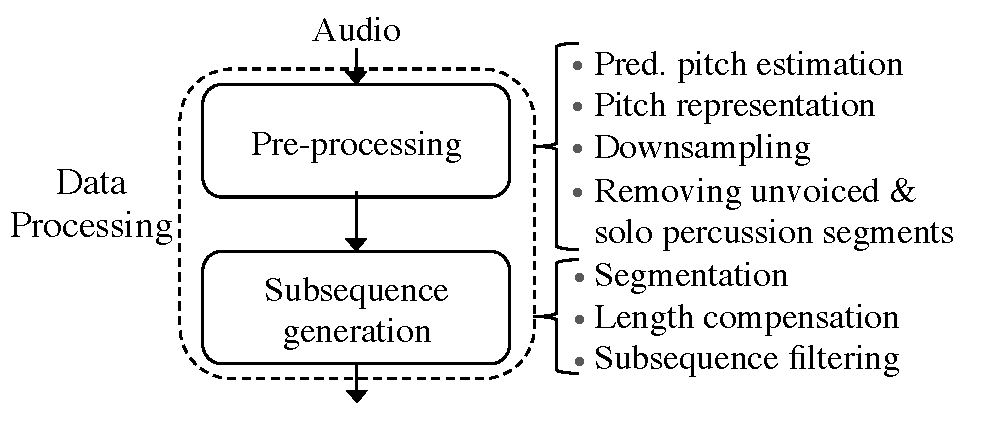
\includegraphics[width=\figSizeEightyFive]{ch06_patterns/figures/discovery/blockDiagram_DataProc.pdf}
	\end{center}
	\caption{Block diagram of the data processing block in melodic pattern discovery task.}
	\label{fig:pattern_discovery_preprocessing_block_diagram}
\end{figure}


The steps involved in the pre-processing block are shown in Fig.~\ref{fig:pattern_discovery_preprocessing_block_diagram}. A brief description of each of these steps is given below:

\paragraph{a) Predominant Pitch Estimation and Representation} 

We consider melody as the predominant pitch in the audio signal. For estimating predominant pitch we follow the procedure we used in~\secref{sec:patterns_evaluation_of_similarity_measures}, which is described in detail in~\secref{sec:data_preprocessing_predominant_melody_estimation}. We use a frame size of 46\,ms and a hop size of 4.44\,ms. Noticeably, the predominant pitch estimation we use algorithm also performs voicing detection, which is used in the later part of our data processing methodology to filter unvoiced segments (\figref{fig:pattern_discovery_preprocessing_block_diagram}). We do not perform any post-processing on the estimated pitch contours.

For the pitch representation to be musically relevant, the pitch values are converted from Hertz to Cents (\secref{sec:data_processing_cent_conversion}). In order to compare melodies across different artists and recordings we additionally consider the tonic pitch of the lead artist in the recording as the reference frequency during this conversion. The tonic of the lead artist for each recording in the collection is identified automatically using a classification-based multi-pitch approach~\citep{salamon2012multipitch}, which is found to be the best performing approach for this task (\secref{sec:data_preprocessing_tonic_identification}).

In the new variant of this method we post-process the predominant pitch contours as described in~\secref{sec:data_preprocessing_pitch_postprocessing}. We perform median and Gaussian filtering to remove spurious pitch jumps lasting over a few samples and to smooth the pitch contours. In addition, we also interpolate short non-voiced segments that usually correspond to intra-phrase breath pauses or to consonants in the lyrics (\secref{sec:data_processing_pitch_interpolation}). 


\begin{figure}
	\begin{center}
		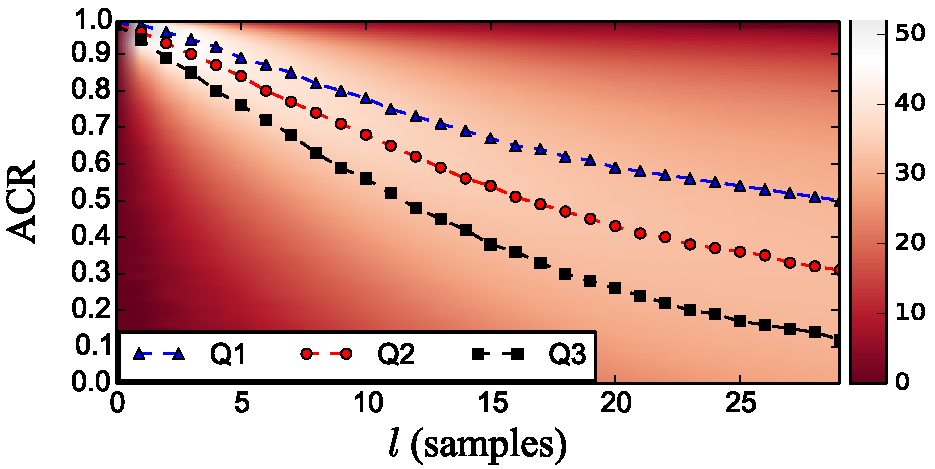
\includegraphics[width=\figSizeEightyFive]{ch06_patterns/figures/discovery/ACRHistogram.pdf}
	\end{center}
	\caption{Histograms of ACR values (histogram value is indicated by the colormap on the right; for ease of visualization, we compress the range of the histogram values by taking its fourth root). Q1, Q2 and Q3 denote the three quartile boundaries of the histogram. }
	\label{fig:ACRHistogram}
\end{figure}


\paragraph{b) Downsampling}

As mentioned above, we estimate predominant pitch at a sampling rate of around 225\,Hz. However, in order to reduce the computational cost, we downsample the predominant pitch sequence \figref{fig:pattern_discovery_preprocessing_block_diagram}. We could not find any study that systematically reports the effect of sampling rate on melodic similarity in \gls{iam}. In such a case, we derive an optimal sampling rate by analyzing the autocorrelation (ACR) of short-time pitch segments generated using a sliding window of 2\,s. We compute the ACR of all possible pitch segments in the entire dataset for different lags $l$, $l\in \lbrace0,1,\dots30\rbrace$, and examine the histogram of normalized ACR values at each lag (\figref{fig:ACRHistogram}). We select the lag at which the third quartile Q3 has an ACR value of 0.8, which corresponds to a sampling rate of 22.22\,ms~(or 45\,Hz). We informally found that this sampling rate generally preserves melodic nuances and rapid pitch movements in Carnatic music while reducing the computational requirements of the task. 

In the new variant of this method, we use the optimal sampling rate derived from our comprehensive quantitative evaluations in~\cite{gulati_ICASSP2015} (see~\secref{sec:patterns_evaluation_of_similarity_measures}). We use a sampling rate of 56\,Hz for Carnatic music and 45\,Hz for Hindustani music.  

%Note that the study in this section was originally presented in~\cite{gulati_SITIS_2014} and was conducted before we quantitatively assessed the optimal parameter settings in~\cite{gulati_ICASSP2015} (see~\secref{sec:patterns_evaluation_of_similarity_measures}). In the subsequent studies  Although, the heuristically chosen sampling rate in this study is not drastically different from the optimal sampling rate reported in~\cite{gulati_ICASSP2015} (see \TODO{Figure(where we show the accuracy vs sampling rate)}). 


\paragraph{c) Solo Percussion Removal} 

As described in \secref{sec:pre_processing_tani_segmentation}, a concert of Carnatic music typically contains a solo percussion section, referred as \gls{tani}, which can last up to 2-25\,minutes. Predominant pitch estimation algorithm employed in this study tracks pitch corresponding to the \gls{mridangam} strokes instead of detecting \gls{tani} sections as non-voiced segments. This poses a challenge for melodic pattern discovery as there are several repeating percussion patterns in \gls{tani} sections, which are often discovered as the closest melodic pattern pairs. In \secref{sec:pre_processing_tani_segmentation} we explain this issue in detail and describe a classification-based approach to detect \gls{tani} sections in audio recordings of Carnatic music. Once detected, we can simply discard the pitch samples corresponding to these sections and overcome the challenge. In addition to avoiding the unwanted melodic patterns being present in the output, by discarding pitch samples from the \gls{tani} sections we also reduce the computational complexity of the pattern discovery task.


\subsubsection{Subsequence Generation}
\label{sec:subsequencegeneration}

In this step we aim to generate melodic pattern candidates from the resultant pitch representation. The steps involved in generating candidate subsequences are as follows:

\paragraph{a) Segmentation} 

As seen in~\secref{sec:patterns_melodic_similarity_results_discussions}, an accurate segmentation of melodic patterns has a big impact on the computation of melodic similarity, and eventually on the retrieval accuracy of melodic patterns. In the literature (Section \TODO{XX}) there are several models proposed for melodic segmentation~\citep{Cambouropoulos2006,muller2009robust,cambouropoulos2001local}. \cite{pearce2008comparison} and \cite{rodriguez2014comparing} provide a comparison of a number of such models. Due to the lack of such studies and reliable models for segmentation of melodic patterns in \gls{iam}, we use brute-force approach for generating pattern candidates. We generate candidate pitch subsequences by using a sliding window of length $W_l$ with a hop size of one sample (22\,ms). Given no quantitative studies investigating the length of the melodic patterns in Carnatic music, we make a choice of $W_l = 2$\,s based on recommendations from a few Carnatic musicians.

Since unvoiced segments are removed from the pitch sequence at the pre-processing step, a window can include pitch samples separated by more than $W_l$ seconds. To handle these cases, we use the time stamps of the first sample ($T_1$) and the last sample ($T_2$) in a window. We filter out all subsequences for which $T_2-T_1 > W_l + \Phi$. We select $\Phi =0.5$\,s to account for the short pauses during a phrase rendition. This value was empirically set to differentiate between inter- and intra-phrase pauses. 

In the new variant of this method, the processing step described in the previous paragraph becomes redundant, and is therefore not applied. Since in this variant the short-duration unvoiced regions in the predominant pitch contours are interpolated, there will not be any situation where $T_2-T_1 > W_l + \Phi$. 


\paragraph{b) Subsequence Filtering} 

One of the challenges in melodic pattern discovery is the presence of combinatorial redundancy in the form of musically trivial patterns in the output~\citep{Lartillot2005}. One such redundancy in our case is that of a melodic pattern comprising a single \gls{svara}. Instead of removing such musically uninteresting patterns after they are discovered, we detect and discard such subsequences (or pattern candidates) during the pre-processing step (\figref{fig:pattern_discovery_preprocessing_block_diagram}). The criterion for discarding such subsequences is summarized below:

\begin{equation}
\label{eq:flatness_measure}
\beta =\sum_{i=0}^{W_n} \Theta\left(S_i\geq T_{\text{std}}\right),
\end{equation}


\noindent where $\beta$ is the flatness measure of a subsequence, $W_n$ denotes its number of samples, $\Theta(z)$ is a Heaviside step function yielding $\Theta(\text{true})\!=\!1$ and $\Theta(\text{false})\!=\!0$, and $S_i$ is the standard deviation at the $i$-th sample of a subsequence, computed using a window of length $W_{\text{std}}$ centered at sample $i$. The threshold $T_{\text{std}}$ determines if a sample belongs to a flat region or not. In order to determine the optimal values of $W_{\text{std}}$ and $T_{\text{std}}$, we manually labeled a number of regions in pitch contour as `flat' and `non-flat' for 4 excerpts in our database. We iterated over different parameter values and analyzed the resultant ROC curve shown in~\figref{fig:ROC_pattern_discovery}). %In  we show the ROC curve obtained for $W_{\text{std}} \in \lbrace100,200,400\rbrace$\,ms. 
Doing so, we found that $W_{\text{std}}=200$\,ms resulted in the best performance and that the knee of the curve corresponded to $T_{\text{std}}=45$\,Cents. Having a value of $\beta$ for each subsequence, we finally filter out the ones for which $\beta \leq \gamma W_n$, using $\gamma = 0.8$. The latter was set by visual inspection.

\begin{figure}
	\begin{center}
		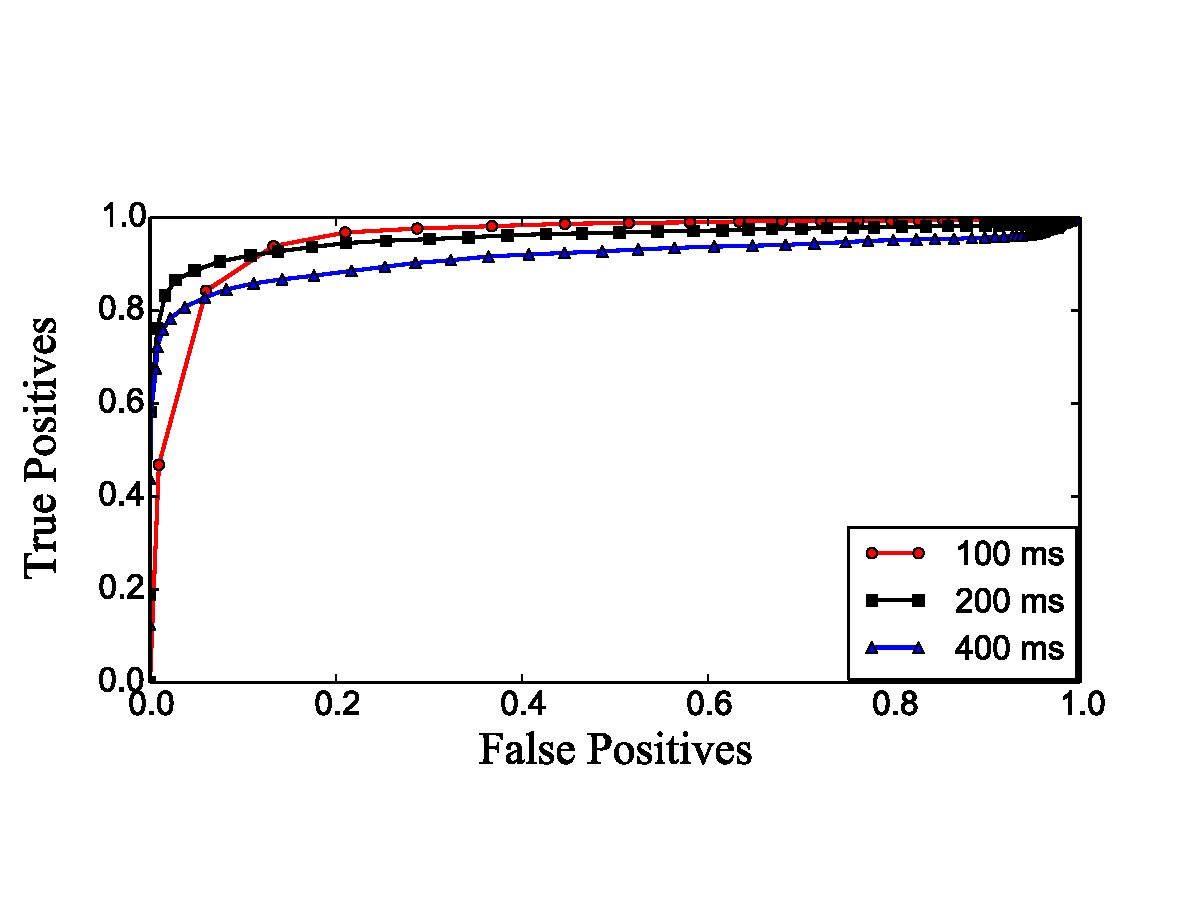
\includegraphics[width=\figSizeEightyFive]{ch06_patterns/figures/discovery/ROCFlatness.pdf}
	\end{center}
	\caption{ROC curves for `flat' and `non-flat' region classification for different values of window length ($W_{\text{std}}$) used for selecting an optimal value of standard deviation $S_i$.}
	\label{fig:ROC_pattern_discovery}
\end{figure}

In the new variant of this method, we use the segmentation approach described in~\secref{sec:nyas_svara_segmentation_method} to detect the stable \gls{svara} regions in melodies. The pitch samples in a subsequence that correspond to these stable \gls{svara} regions are regarded as `flat', which is analogous to $S_i\geq T_{\text{std}}$ being `True' for those samples. All other parameters remain the same as described above. This change is done because the segmentation approach produces more reliable estimates of the stable melodic regions compared to the simple measure using local standard deviation of the pitch samples. 

 %In the current study our dataset comprises only Carnatic music. For Hindustani music the reduction ratio of number of pattern candidates might be even higher due to the presence of long held \gls{svaras}.

\subsubsection{Intra-recording Pattern Discovery}
\label{sec:intraRecordingPatternDiscovery}

In this step our aim is to discover melodic patterns within each recording in the audio collection. We perform an exact pattern discovery by computing the similarity between every possible subsequence pair obtained within an audio recording. Thus, the computational complexity of this task is quadratic ()$\mathcal{O}(n^2)$) over the number of subsequences. We regard the top $N=25$ closest subsequence pairs in each recording as seed patterns. We omit overlapping subsequences in order to avoid trivial matches and additionally constrain the top $N$ seed pattern pairs to be mutually non-overlapping. Due to this constraint for some recordings we obtain less than 25 pattern pairs. 


\paragraph{Melodic Similarity} 

We compute melodic similarity between two subsequences using a \gls{dtw}-based distance measure~\cite{Sakoe78TASLP} (Section\TODO{XXX}). This choice is supported by our findings in~\secref{sec:patterns_melodic_similarity_results_discussions}, wherein we showed that a \gls{dtw}-based distance measure outperforms Euclidean distance measure in melodic similarity computation in \gls{iam}. We use a step condition of $\lbrace(1,0), (1,1), (0,1)\rbrace$ and the squared Euclidean distance as the cost function (Section\TODO{XXX}). We do not use any penalty for insertion and deletion. In addition, we apply the Sakoe-Chiba global constraint with the band width set to 10\% of the pattern length. This constraint was found to be sufficiently large for accounting time warpings in melodic repetitions in Carnatic music (see \tabref{tab:melodic_similarity_results}). For the case of Hindustani music, an unconstrained \gls{dtw} variant is shown to perform the best. However, due to the computational complexity of the task, in order to make it computationally feasible we finally choose 10\% band width for both the music traditions. Notice that these parameter values are close to the optimal settings but not the most optimal settings for a \gls{dtw} variant that we obtained in \secref{tab:melodic_similarity_results}. We make these choices in order to allow lower bounding as explained in the subsequent sections. 

\TODO{Should we copy the DTW equation here, or show an example of aligned pattern. Or atleast say how is dtw taking care of local time variations.}
	

\paragraph{Lower Bounding \gls{dtw}}
\label{LowerBoundingDTW}

The computational complexity of a brute-force pattern discovery system using a \gls{dtw} distance measure is quadratic ($\mathcal{O}(n^2)$) over both the number of subsequences and the length of a subsequence. For a dataset as big as ours that contains millions of subsequences (pattern candidates), where the length of each subsequence is around 100\,samples, the system becomes extremely demanding in terms of the CPU time. Even after reducing the number of pattern candidates by filtering out subsequences in the pre-processing step and reducing the length of the subsequences by downsampling the pitch representation, it is not practically feasible to perform the task. One of the ways to address this problem is to use indexing or lower bounding techniques with which we can prune subsequence pairs that can not possibly be the best matches. Pruning of the subsequence pairs reduces the number of times the \gls{dtw} computation is done, and thus make \gls{dtw} distance computations tractable for datasets with large number of subsequences.

In literature there are several methods proposed for indexing the \gls{dtw} distance~\citep{Keogh2004,vlachos2003indexing}. These methods differ in terms of their computational complexities and the type of indexing techniques they employ (approximate or exact). In this study to speed up \gls{dtw} computations we use the exact \gls{dtw} indexing technique~\citep{Keogh2004} and apply cascaded lower bounds as explained in~\cite{Rakthanmanon2013}. This method is parameter free, it does not require any pre-processing of the data and there is no constraint on the minimum and maximum query length. In particular, we use FL (first-last) lower bound and LB\_Keogh bound for both query to reference and reference to query matching. Besides, we apply early abandoning, both during the computation of lower bounds as well as during the \gls{dtw} distance computation. These lower bounding and early abandoning techniques are explained in section XXX, however, for a more detailed explanation we refer to~\cite{Rakthanmanon2013}. 

In \algoref{alg:algorithmdiscovery} we show the pattern discovery routine that uses cascaded lower bounds to speed up \gls{dtw}. This pseudo-code provides a better understanding of the pruning procedure and puts in context the utility of using different lower bounds. Note that in this routine we show the discovery of only the closest subsequence pair. With a trivial addition of incorporating a priority queue that stores the K most closest subsequence pairs at each step, we extend it to our use-case of discovering the top K closest melodic patterns. We further optimize this routine by pre-computing the subsequence envelopes used in the computation of LB\_Keogh bound section XXX.

\renewcommand{\algorithmiccomment}[1]{\bgroup\hfill\tiny//~#1\egroup}
\begin{algorithm}
\caption{Discovering the closest subsequence pair using the \gls{dtw} distance and cascaded lower bounds.}
\label{alg:algorithmdiscovery}
	\begin{algorithmic} 
	
	\State {\bf Input:} array $\mathrm{S}$ containing $N$ number of subsequences
	\State \texttt{best\_so\_far} = \texttt{infinity};
	\For{$i$=0; $i \leq N-1$; $i$++}
		\For{$j$=0; $j \leq N-1$; $j$++}
			\State  \texttt{dist\_FL} = \texttt{LB\_KIM\_FL($\mathrm{S}_i$, $\mathrm{S}_j$)}			
			\If {\texttt{dist\_FL} < \texttt{best\_so\_far}}				
				\State  \texttt{dist\_EQ} = \texttt{LB\_Keogh($\mathrm{S}_i$, $\mathrm{S}_j$)}				
				\If {\texttt{dist\_EQ} < \texttt{best\_so\_far}}				
					\State  \texttt{dist\_EC} = \texttt{LB\_Keogh($\mathrm{S}_j$, $\mathrm{S}_i$)}					
					\If {\texttt{dist\_EC} < \texttt{best\_so\_far}}					
						\State  \texttt{true\_dist} = \texttt{DTW($\mathrm{S}_i$, $\mathrm{S}_j$)}						
						\If {\texttt{true\_dist} < \texttt{best\_so\_far}}
							\State \texttt{best\_so\_far} = \texttt{true\_dist}
							\State \texttt{closest\_pair\_index} = ($i$,$j$)							
						\EndIf
					\EndIf
				\EndIf
			\EndIf
		\EndFor
	\EndFor
	
	\end{algorithmic}
\end{algorithm}
				

\paragraph{Pattern Length Compensation}
\label{PatternLengthCompensation}

Along with the local non-linear time warpings, the overall length of a melodic pattern may also vary across repetitions. For example, a melodic pattern of length 2\,s might be sung in 2.2\,s in a different position in the recording. We handle this by using multiple time scaled versions of a subsequence in the distance computation. This technique is also referred to as local \gls{dtw} and is shown to have tighter lower bounds~\citep{Zhu2003}. It should be noted that such issues are typically addressed by using a subsequence variant of the \gls{dtw} distance measure. However, the lower bounding techniques we use to speed up the \gls{dtw} distance computation do not work for the subsequence variant of the \gls{dtw}. 

For every subsequence, we generate five subsequences by uniformly time scaling it by a factor of $\alpha \in I_{\text{intp}} =\lbrace 0.9, 0.95, 1, 1.05, 1.1\rbrace$, such that the length of the resulting subsequences is $W_l$. We use cubic interpolation for uniformly time scaling a subsequence. Creating five uniform time scaled subsequences for each subsequence increases the computational cost by a factor of 25. We observe that the distance between a subsequence pair $X_{1.0}$ and $Y_{1.05}$ is very close to the distance between the pair $X_{1.05}$ and $Y_{1.1}$ (the sub-index denotes the interpolation factor $\alpha$). Thus by following this rationale and using this approximation, we can avoid the distance computation between 16 of the 25 combinations without a significant compromise on accuracy. We only retain the combinations for which the difference between the interpolation factors of subsequence pairs are unique. \TODO{Figure?? matrix if time permits}

\subsubsection{Inter-recording Pattern Detection}
\label{sec:inter_recording_pattern_search}

After discovering melodic patterns within each audio recording, we now proceed to detect their occurrences in all the recordings in the collection. For this, we consider every seed pattern as a query and perform an exhaustive search over all the subsequences obtained from the entire audio music collection. For every seed pattern we store top $M=200$ closest matches (referred to as search patterns). To avoid redundancy in the search results, we constrain search patterns for every seed pattern to be mutually non-overlapping. Similar to the intra-recording pattern discovery step, here also for every subsequence we consider 5 uniformly  time scaled subsequences in the distance computation. Furthermore, for detecting occurrences of seed patterns in other recordings we use the same similarity measure and lower bounding techniques as used in ~\secref{sec:intraRecordingPatternDiscovery}. The pattern detection routine is a small modification of the routine shown in~\algoref{alg:algorithmdiscovery}. Instead of a single subsequence array, we would have two arrays; one of which comprises the seed patterns (queries) and the other comprises subsequences obtained from all the recordings (target candidates). 

\subsubsection{Rank Refinement}
\label{sec:rankRefinement}

As mentioned before, the lower bounds used for speeding up the distance computations are not valid for any variant of the \gls{dtw} distance. This constraint governed the choices made for the \gls{dtw} variant and the parameter settings for computing melodic similarity in both the intra and the inter-recording pattern processing blocks. However, once the top matches are found, nothing prevents us from reordering the ranked list using any variant of the \gls{dtw} distance. This is because the number of top matches we consider ($M=200$) per query is orders of magnitude smaller than the total number of subsequences obtained from the entire audio collection. For every query pattern, we now recompute the melodic similarity with its top M search patterns using a more robust and a better performing variant of the \gls{dtw} distance.

During rank refinement, we select a \gls{dtw} step condition of $\lbrace(1,2), (1,1), (2,1)\rbrace$ to avoid some pathological warpings of the path. This step condition, which also acts as a local constraint was shown to better model the melodic similarity in~\secref{sec:patterns_melodic_similarity_results_discussions}. Furthermore, we investigate four different distance measures $d_i$, $i=1,\dots 4$, used in the computation of the \gls{dtw} cost matrix. These distance measures are described below in~\eqref{eq:distance_measures_discovery}. For a better understanding of the distance measures we show them in~\figref{fig:Distances_DTW_discovery}.
%We choose $d_1 = \delta^2$, $d_2=\delta$, $d_3 = \delta-25$ if $\delta>25$ or %$d_3=0$ otherwise, $d_4 = (\delta-\phi)^{1.5} + \varphi$ if $\delta>100$ or $d_4 %= d_3$ otherwise. 


\begin{figure}
	\begin{center}
		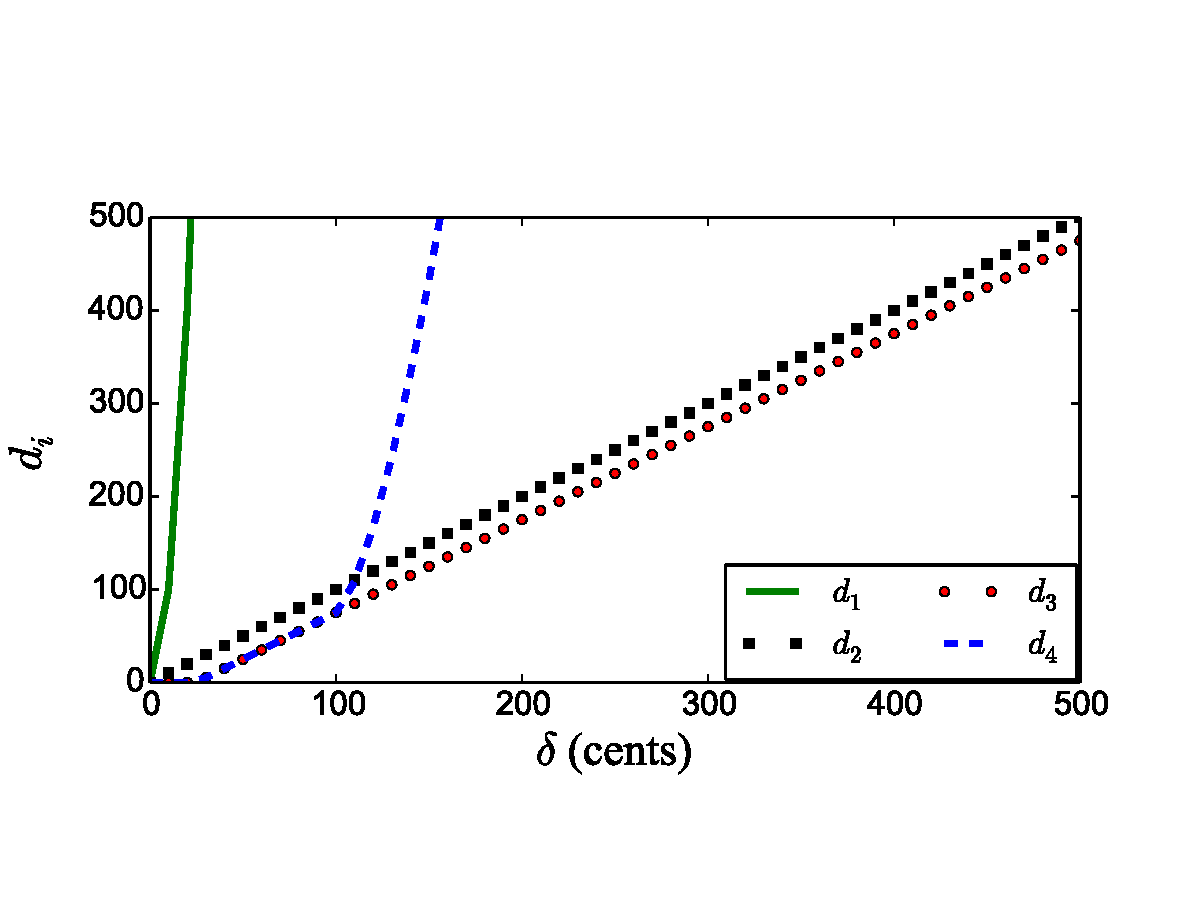
\includegraphics[width=\figSizeEightyFive]{ch06_patterns/figures/discovery/distances.pdf}
	\end{center}
	\caption{Output of four distance measures as a function of cityblock distance $\delta$. }
	\label{fig:Distances_DTW_discovery}
\end{figure}


\begin{equation}
\begin{aligned}
d_1& = \delta \hspace{.5em};&
d_3& = 
\begin{cases}
\delta-25, & \hspace{1cm} \text{if } \delta >25\\
0, & \hspace{1cm}\text{otherwise } 
\end{cases}
\\
d_2& = \delta^2 \hspace{.5em};&
d_4 &= 
\begin{cases}
(\delta-\phi)^{1.5} + \varphi, & \text{if } \delta >100\\
d_3, & \text{otherwise}
\end{cases}
\end{aligned}
\label{eq:distance_measures_discovery}
\end{equation}

\noindent where $\delta = |p_1-p_2|$ is the city block distance between two pitch values and all numeric values are in Cent scale. We set $\phi =99.555$ and $\varphi = 74.7$ to maintain point and slope continuity of the function. The formulation for these different distance measures ($d_i$) is inspired by our own experience and some of the approaches we find in the literature~\citep{Ishwar2013,Rao2014}. We denote the four variants of the rank refinement method by $V_i$, $i=1\dots 4$.


\subsection{Evaluation}

\subsubsection{Music Collection}
\label{sec:pattern_discovery_musiccollection}

The music collection used for studying the task of pattern discovery in this section comprises 365\,hours Carnatic music. It contains 1764 audio recordings, which are carefully compiled as a part of the CompMusic Carnatic music corpus (\secref{sec:corpus_carnatic_music_corpus}). As explained in~\secref{sec:corpus_carnatic_music_corpus}, these audio recordings are ripped from commercially released music CDs. The selected music material is diverse in terms of the number of artists, gender of lead artists, number of different \glspl{raga}, year of release and various forms within Carnatic music.

\TODO{If time permits provide statistics of this dataset}


\subsubsection{Evaluation Methodology}
\label{sec:evaluationmethodology}

One of the challenges in an unsupervised data-driven approach such as the one we use for discovering melodic patterns is evaluation. We here perform a quantitative evaluation based on expert feedback. For the entire dataset we obtain over 15\,million search patterns for each of the rank refinement methods. We divide seed patterns into three categories based on the distance between the seed pairs, which we denote by $D$. The distribution of the distance $D$ between the seed pattern pairs is shown in~\figref{fig:SeedPatternsDistanceDistribution}. Then, to have an equal representation from the range of values of $D$, 200 seed pairs equally distributed among these categories are randomly selected for evaluation. Seed category boundaries are $\mu \pm 1.5\sigma$, where $\mu$ and $\sigma$ are the mean and the standard deviation of the distribution of $D$. For every selected seed pattern we consider the first 10 search patterns for each of the four rank refinement methods for evaluation. Thus, in total, we obtain 200 seed pairs and 8,000 search patterns for expert evaluation.

Expert evaluation is performed by a professional Carnatic musician who has received over 20 years of music education. For examining similarity between two melodic patterns, the musician listened to the audio fragments corresponding to these patterns and scored a 0 for melodically dissimilar and a 1 for melodically similar pattern. The musician annotated melodic similarity for each seed pair and between the seed and its search patterns for every rank refinement method.


\begin{figure}
	\begin{center}
		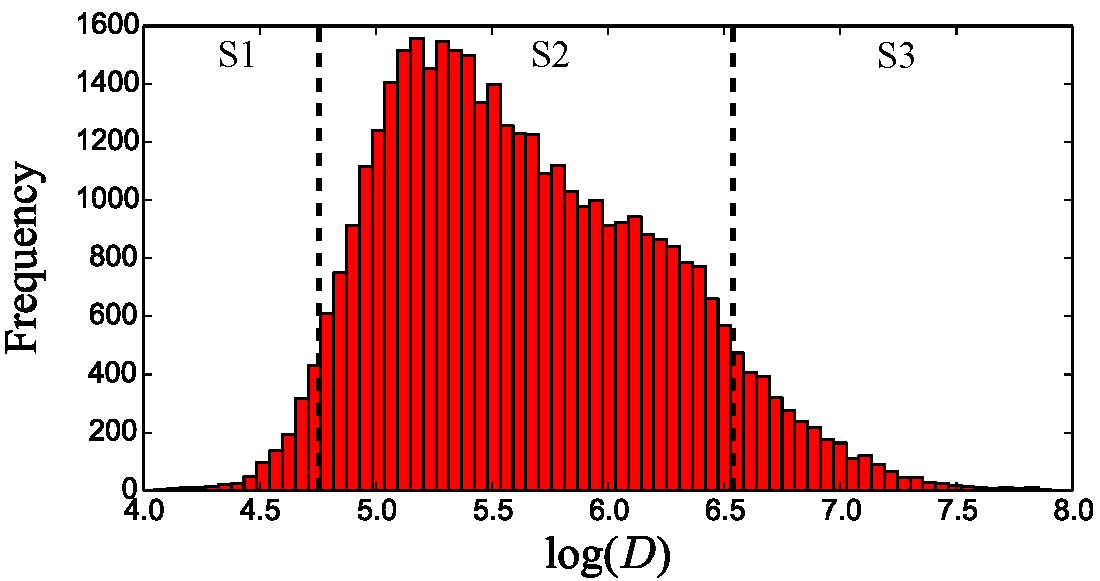
\includegraphics[width=\figSizeEightyFive]{ch06_patterns/figures/discovery/SeedDistribution.pdf}
	\end{center}
	\caption{Distance distribution of seed patterns. Three seed pattern categories are marked by S1, S2 and S3.}
	\label{fig:SeedPatternsDistanceDistribution}
\end{figure}


To quantify the musician's assessment of the similarity between the melodic patterns  we use \gls{map}, a typical evaluation measure in information retrieval~\citep{manning2008introduction}, which is also very common in \gls{mir}. This way, we have a single number to evaluate the performance of the four different rank refinement methods. Since we do not have ground-truth annotations of melodic patterns for our dataset, total number of occurrences of different patterns is unknown. Therefore, while computing the \gls{map} scores we consider the total number of relevant patterns as the number of relevant patterns retrieved in the top 10 search results.  For assessing statistical significance we use the Mann-Whitney U test~\citep{mann1947test} with $p < 0.05$. To compensate for multiple comparisons, we apply the Holm-Bonferroni method~\citep{holm1979simple}. Thus, eventually we use a much more stringent criteria than $p < 0.05$ for measuring statistical significance. We also use ROC curves to analyze the separation between the distance distribution of melodically similar and dissimilar subsequences~\citep{manning2008introduction}. 


\subsection{Results and Discussion}
\label{sec:patterns_discovery_results}

Before presenting the results of the evaluation of the discovered patterns, we provide details in terms of the number of patterns and \gls{dtw} computations done at each step. Our dataset comprising 365\,hours of audio data contains nearly 300\,million pitch samples (considering 225\,Hz as the sampling rate of the pitch contours). In a brute force segmentation scenario that would amount to roughly the same number of pattern candidates. However, since we downsample the pitch contours and filter out musically trivial patterns, we retain around 17.5\,million pattern candidates (subsequences) after data pre-processing step. In the intra-recording pattern discovery block, for all the recordings, nearly 1.41\,trillion distance computations are done to obtain 79,172 seed patterns. In the inter-recording pattern detection block, nearly 12.42\,trillion distance computations are done to obtain 15 million search patterns for each variant of the rank-refinement method. These numbers give us an idea about the computational complexity of the task and shows the scale at which this study is performed.

\begin{table} 
	\begin{centering}
		\begin{tabular}{ c | c c }
			\tabletop
			Lower bound   	& Intra-rec.(\%)		&	Inter-rec.(\%) \\	
			\tablemid
			LB\_KIM\_FL   	& 52	&	45 \\	
			LB\_Keogh\_EQ   	& 23	&	51 \\
			LB\_Keogh\_EC   		& 1	&	3 \\
			\tablebot
		\end{tabular}
		\caption{Percentage of exits after a lower bound computation with respect to the total number of distance computations.}
		\label{tab:computationalStats}	
		\par \end{centering}	
\end{table}

We now analyze the contribution of different lower bounds in pruning the search space. In~\tabref{tab:computationalStats} we show in percentage the number of times the program counter exits after a lower bound computation with respect to the total number of distance computations. As mentioned before, the total number of distance computations are 1.41\,trillion for intra-recording pattern discovery and 12.42\,trillion for inter-recording pattern detection. From~\tabref{tab:computationalStats} we see that the \gls{dtw} computation is avoided in 76\% and 99\% of the distance computations done in the intra-recording pattern discovery and the inter-recording pattern detection task, respectively. It is evident that the lower bounding methods are more effective in the former case compared to the latter. This is expected as different songs may correspond to different \glspl{raga} and hence use different set of musical notes. An interesting observation here is that LB\_KIM\_FL (first-last) lower bound whose computational complexity is $\mathcal{O}(1)$ prunes nearly 50\% of the total numbers of possible subsequence pairs. 

\begin{figure}
	\begin{center}
		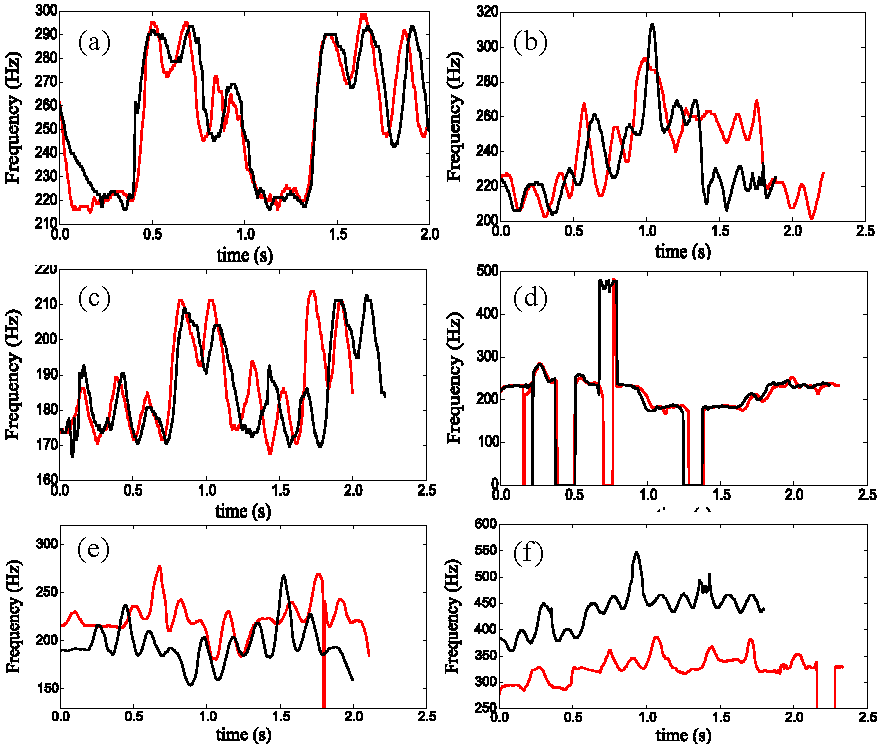
\includegraphics[width=\figSizeHundred]{ch06_patterns/figures/discovery/combinedPatterns.pdf}
	\end{center}
	\caption{Examples of the discovered melodic patterns.}
	\label{fig:combinedPatternsDiscovered}
\end{figure}

To demonstrate the capabilities of the approach, we show a few examples of the discovered melodic patterns in~\figref{fig:combinedPatternsDiscovered}. Our approach robustly extracts patterns in different scenarios such as large local time warpings~(b), uniform scaling~(c), patterns with silence regions~(d) and across different tonic pitches~(e and f). It is worth mentioning that, during the process of annotation, the musician found several musically interesting results. For example, striking similarity between phrases of two different \glspl{raga}, between phrases in sung melodies and the melodies played on instruments (Violin or \Gls{vina}), and phrases sung by different artists. Many of the discovered patterns are the characteristic melodic phrases of the \glspl{raga}, which are the primary cues for \gls{raga} recognition. Overall, we find that the obtained results are musically relevant and can be used to establish meaningful relationships between audio recordings. We explore the usability of these discovered patterns in the task of automatic \gls{raga} recognition in~\secref{sec:phrase_based_feature_extraction}.

We now present our formal evaluations. We first evaluate the performance of the intra-recording pattern discovery task. We find that the fraction of melodically similar seed pairs within each seed category S1, S2 and S3 consistently decreases: 0.98, 0.67 and 0.31, respectively. This is expected as the seed categories are created based on the distance ($D$) between the seed pairs. These numbers indicate that the computed distance strongly correlates to the melodic similarity between the patterns. However, from these numbers we do not get much information about the amount of separation between the distance distributions of melodically similar and dissimilar seed pattern pairs. To examine the separation, we compute the ROC curve as shown in~\figref{fig:combinedROCPatternDiscovery} (solid blue line). The knee of the curve corresponds to a precision of approximately 80\% for 10\% of false positive cases. This indicates that the chosen \gls{dtw}-based distance measure is a sufficiently good candidate for computing melodic similarity for the case of intra-recording seed pattern discovery. 


\begin{figure}
	\begin{center}
		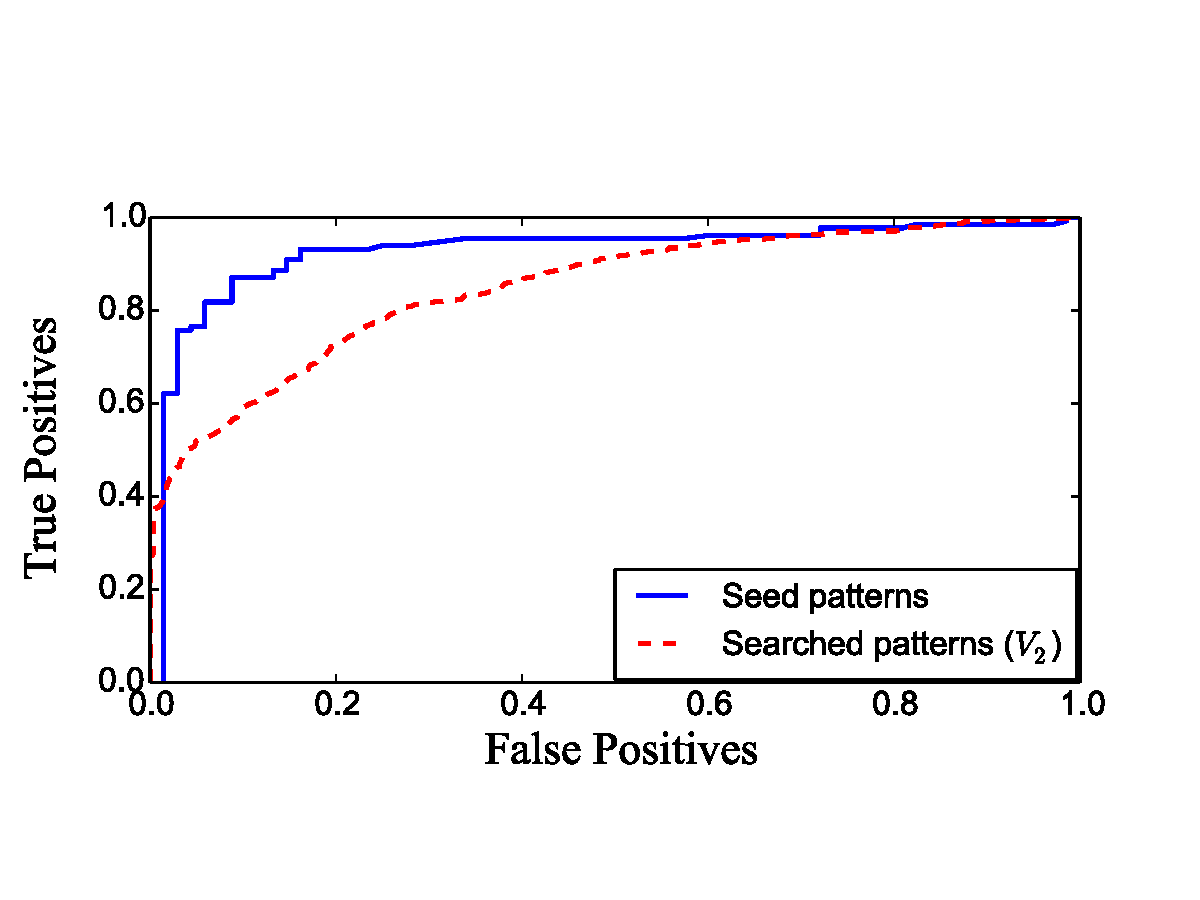
\includegraphics[width=\figSizeEightyFive]{ch06_patterns/figures/discovery/seedROC.pdf}
	\end{center}
	\caption{ROC curve for seed pairs and search patterns (using $V_2$) in the evaluation set.}%\vspace{-1em}
	\label{fig:combinedROCPatternDiscovery}
\end{figure}

\TODO{make the row and colum spacing consistent across tables}
\begin{table} 
	\begin{centering}	
		\begin{tabular}{ c | c c c c}
			\tabletop
			Seed Category   & $V_1$		&	$V_2$ & $V_3$	 &	$V_4$ 	\\	
			\tablemid
			S1 & 0.92    &	0.92		&	0.91    &	0.89\\
			S2 & 0.68    &	0.73		&	0.73    &	0.66\\
			S3 & 0.35    &	0.34    &	0.35    &	0.35\\
			\tablebot
		\end{tabular}
		\caption{MAP scores for four variants of rank refinement method ($V_i$) for each seed category (S1, S2 and S3).}
		\label{tab:meanAveragePrecision_pattern_discovery}
		\par \end{centering}	
\end{table}

\begin{figure}
	\begin{center}
		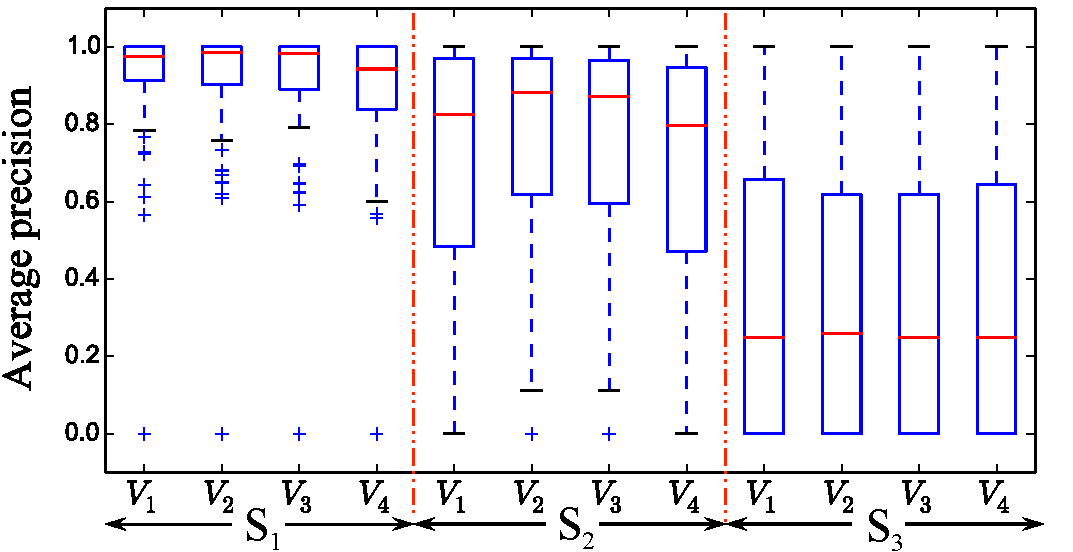
\includegraphics[width=\figSizeHundred]{ch06_patterns/figures/discovery/boxPlot.pdf}
	\end{center}
	\caption{Boxplot of average precision values for the different variants of the rank refinement method ($V_i$) for each seed category. }
	\label{fig:boxPlotMAPPatternDiscovery}
\end{figure}

Next, we evaluate the performance of inter-recording pattern detection task and assess the effect of the four \gls{dtw} cost variants explained in~\secref{sec:patterns_discovery_results} (denoted by $V_1 \dots V_4$). To investigate the dependence of the performance on the category of the seed pair, we perform the evaluation within each seed category. In~\tabref{tab:meanAveragePrecision_pattern_discovery} we show the \gls{map} scores obtained for the different variants of the rank refinement method ($V_1, V_2, V_3$ and $V_4$) for each seed category (S1, S2 and S3). In addition, we also present a box plot of corresponding average precision values in~\figref{fig:boxPlotMAPPatternDiscovery}. In general, we observe that every method performs well for category S1, with a MAP score around 0.9 and no statistically significant difference between each other. For category S2, $V_2$ and $V_3$ perform better than the rest and the difference is found to be statistically significant. The performance is poor for the third category S3 for every variant. The difference in performance between any two methods across seed categories is statistically significant. We observe that MAP scores across different seed categories correlate strongly with the fraction of melodically similar seed pairs in that category (discussed above). This means that the seed pattern pairs that have high distance $D$ between them obtain low average precision when used as query patterns and vice-versa. This might be because across repetitions of such patterns there could be a high degree of melodic variation, to model which the current similarity measure appears inadequate. In addition, closely repeating seed pattern pairs (i.e.~with low distance $D$ between them) might have more number of repetitions with low degree of melodic variations, for which the current similarity measure performs well. 

%It suggests that repeating patterns do have some significance, they are not a product of coincidence, and therefore, they are more likely to recur across recordings. Note that we do not imply that every repeating pattern is (equally) musically significant or is a characteristic phrase of a \gls{raga}. There are different types of repeating patterns in melodies of \gls{iam}. The task of characterizing the discovered patterns is addressed in~\secref{sec:patterns_characterization_of_melodic_patterns} \TODO{rehphrase this last part}

Finally, we analyze the distance distributions of melodically similar and dissimilar search patterns. For this we use the best performing rank-refinement variant $V_2$. To examine the separation in the distance distribution, we compute the ROC curve as shown in~\ref{fig:combinedROCPatternDiscovery} (dashed red line). We observe that the separability between melodically similar and dissimilar subsequences in this case is poorer than the one obtained for the seed pairs (solid blue line). This suggests that it is much harder to differentiate melodically similar from dissimilar patterns when the search is performed across recordings. This can be attributed to the total number of melodically dissimilar subsequences (irrelevant documents) for every query subsequence, which is orders of magnitude higher in this task compared to the task of pattern discovery within a recording. In addition, one of the reasons can also be that the melodic phrases of two allied \glspl{raga} \TODO{definition of allied?} are differentiated based on subtle melodic nuances~\cite{Viswanathan2004}. Hence, one faces a much more difficult task, which requires a superior melodic similarity measure. Moreover, some of these melodic nuances might be specific to \glspl{raga}, learning which might be possible only under a supervised framework. 



\subsection{Summary}
\label{sec:patterns_pattern_discovery_summary}

We presented a data-driven unsupervised approach for melodic pattern discovery in large audio collections of \gls{iam}. We first discovered seed patterns within a recording and later used those as queries to detect similar occurrences in the entire dataset. We used DTW-based distance measures to compute melodic similarity and compared four different rank refinement variants. To evaluate the approach we use a sizable music collection comprising 365\,hours of audio recordings of Carnatic music, which represents the diversities present in the music tradition. A randomly sampled subset of the extracted melodic patterns was evaluated by a professional Carnatic musician. We saw that discovering 25 closest seed pattern pairs within each recording and retrieving their 200 closest patterns from the entire music collection resulted in around 12 trillion distance computations. Using cascaded lower bounding techniques for the \gls{dtw} distance we saved nearly 76\% of the total computations for the intra-recording pattern discovery task and around 99\% of the total computations for the inter-recording pattern detection task. Our quantitative evaluation indicated that a DTW-based distance measure performs reasonably well for intra-recording discovery. However, the performance for the inter-recording pattern detection task was inferior suggesting that we require better melodic similarity measures for searching occurrences across recordings. This is a clear direction for future works. We showed that a variant of the \gls{dtw} cost function using cityblock distance performs slightly better than the rest for refining the ranks of the retrieved search results. Qualitative feedback from the musician suggested that the extracted melodic patterns are interesting and musically meaningful and possibly be utilized in higher level computational tasks such as automatic \gls{raga} recognition, and music recommendation and discovery. 

\TODO{ application: Furthermore, the discovered patterns can be utilized in applications for enhanced music listening, exploratory tools for musicologists and in pedagogical tools. Write quite many applications in the intro. Highlight all the possible contexts in which this output can be exploited}

%Our results also indicate that the patterns which find close matches within a recording have a higher average precision when they are queried for their occurrences across recordings.



%################################################################################################################
%########################################### IMPROVING MELODIC SIMILARITY #######################################
%################################################################################################################


\section{Characterization of Melodic Patterns}
\label{sec:patterns_characterization_of_melodic_patterns}

In the previous section we described our approach to discover melodic patterns in sizable audio music collections of \gls{iam}. Our primary goal was to extract as many different types of recurring melodic patterns and as many occurrences of them as possible, irrespective of their musical relevance. Recurring patterns in melodies of \gls{iam} may differ drastically in terms of their musical relevance (Section XX). Their functional role in melodies may vary from being a melodic ornamentation to being a characteristic melodic phrase of a \gls{raga}. Thus, in order to effectively utilize the discovered melodic patterns in different melodic analyses and applications in \gls{iam}, characterization of these patterns in terms of their musical relevance and functional roles is crucial. In addition, since a musically meaningful melodic similarity threshold is unavailable in such an unsupervised analysis (\secref{sec:patterns_discovery_results}), no similarity thresholding is performed. The discovery approach in~\secref{sec:patterns_melodic_pattern_discovery} works with a fixed number of closest pattern matches irrespective of the absolute value of the melodic similarity. As a result of which the output of the pattern discovery approach may contain a large amount of music irrelevant or noisy matches. Although, as seen in~\secref{sec:patterns_discovery_results}, separation between the distance distributions of melodically similar an dissimilar patterns appears favorable (\figref{fig:combinedROCPatternDiscovery}), indicating that an optimal melodic similarity threshold can potentially remove the noisy matches with a reasonable accuracy. 

In this section we address both the issues, determining a meaningful melodic similarity threshold, and characterizing discovered melodic patterns by performing a network analysis. We exploit the topological properties of the network to determine a similarity threshold. For characterizing patterns we first detect non-overlapping communities in the network and then characterize the communities by utilizing the related editorial metadata. As mentioned, repeating patterns in melodies of \gls{iam} can belong to varied categories. In order to reduce the complexity involved in identification and evaluation of different types of melodic patterns, we focus on \gls{raga} motifs, which is arguably the most advantageous pattern category for computational melodic analyses of \gls{iam}. \Gls{raga} motifs as defined in SEction \TODO{XX} are characteristic melodic patterns of \glspl{raga}, which are the prominent cues exploited by both performers and listeners for depicting and identifying \glspl{raga} in \gls{iam}. \Gls{raga} motifs are learned quite explicitly through years of musical training, and they provide a base for artists' to improvise. Due to these reasons \gls{raga} motifs are distinctly recognized by performing musicians. In addition, such melodic patterns are crucial for \gls{raga} based music retrieval systems, automatic \gls{raga} recognition, studying similarities between artists and recordings, and in developing pedagogical tools for \gls{iam}. Due to these factors we choose \gls{raga} motifs to study the task of characterization of melodic patterns.  

\TODO{State of the art?}


\subsection{Method}

To recapitulate, we address the task of discovering \gls{raga} motifs in audio music collections of \gls{iam}. The block diagram of the proposed approach is shown in~\figref{fig:block_diagram_characterization}. There are two main processing blocks: (a) melodic pattern discovery and (b) pattern characterization. Both these blocks are described at length in the subsequent sections.

\begin{figure}
	\begin{center}
		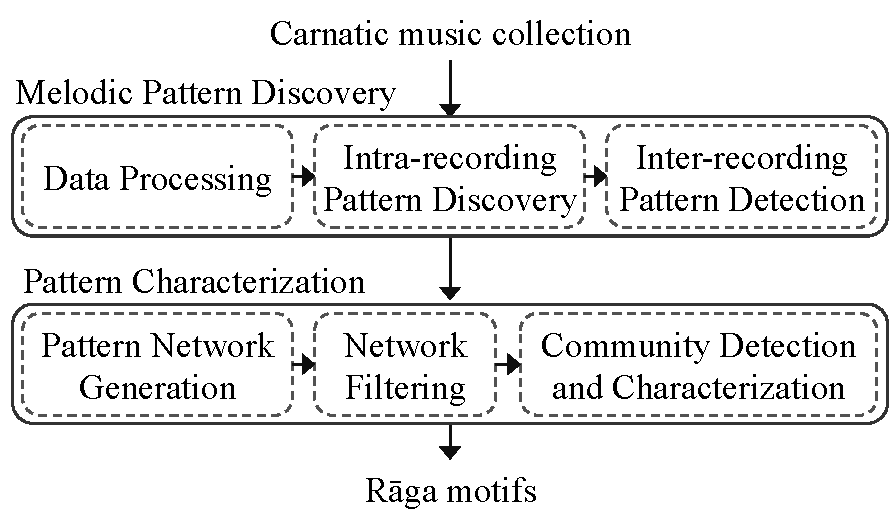
\includegraphics[width=\figSizeHundred]{ch06_patterns/figures/Characterization/blockDiagram.pdf}
	\end{center}
	\caption{Block diagram of the proposed approach for characterizing melodic patterns.}
	\label{fig:block_diagram_characterization}
\end{figure}


\subsubsection{Melodic Pattern Discovery}
\label{sec:patterns_characterization_pattern_discovery}

As mentioned, discovering melodic patterns in a sizable audio collection of \gls{iam} is a challenging task. To get a reliable input for our approach, we employ the pattern discovery approach we describe in~\secref{sec:patterns_melodic_pattern_discovery}. This is one of the few unsupervised systems, we are aware of, that can discover meaningful melodic patterns in large-scale collections of \gls{iam}. Recall that the output of our pattern discovery approach comprises seed patterns, which are discovered within the recordings, and also, their nearest neighbors in the entire audio collection. In this study, we extract the top 25 closest seed pattern pairs from every recording and consider the top 20 closest patterns for each seed pattern across the recordings. \TODO{is this the top XX closest correct?}. We use the same parameter settings and the implementation of the method as described in~\secref{sec:patterns_melodic_pattern_discovery}. 

Notice that the output of our melodic pattern discovery system may contain a high degree of redundancy in terms of overlapping patterns. This is despite the constraints to only select mutually non-overlapping patterns during the discovery and search phase. This redundancy arises primarily because we perform the inter-recording pattern search for each pattern in the seed pair. Since seed pair patterns are (often) close repetitions of each other, we end up retrieving nearly the same set of patterns as nearest neighbors for both of them. Thus, there exists a large number of overlapping patterns in the output of our pattern discovery block. We chose to perform inter-recording pattern search for each pattern in the pair separately as it exploits intra-class variability present in the patterns, which might provide better retrieval results \TODO{Ask Joan a ref for this}. 

We reduce redundancy in the output of pattern discovery system by following a simple procedure. For every discovered melodic pattern we search for its closest pattern across all the recordings using the same similarity measure as used in the intra-recording pattern discovery block. For each recording we parse a list of patterns in that recording sorted in the increasing order of their distances from their closest patterns. While parsing the list we remove every pattern for which there exists an overlap with another pattern placed higher (lower index) in the sorted list. Thus, at the end of this process we retain only non-overlapping patterns in every recording.



\subsubsection{Melodic Pattern Characterization}
\label{pattern_characterization}

Before we formally describe this processing step, we provide the underlying intuition behind it. As explained earlier, a discovered melodic pattern obtained from the previous step can correspond to either a \gls{raga} motif, a composition-specific motif or to a \gls{gamaka} pattern (Section \TODO{secref}). Our objective is to characterize the discovered patterns in order to identify the ones that are \gls{raga} motifs. The information available to accomplish this task is; a bunch of melodic patterns, pitch sequences corresponding to the patterns, editorial metadata of the recordings to which the patterns belongs and the location of the patterns in the recordings. If we take a single melodic pattern, the only possible indicator of its category could be the characteristics of its pitch sequence. However, to the best of our knowledge (acquired from published studies and discussions with musicians), \gls{raga} motifs do not possess any peculiar pitch characteristics in general. Therefore, characterization of the discovered melodic patterns considering one pattern at a time under unsupervised scenario appears to be virtually impossible. Such melodic motifs are explicitly learned for each \gls{raga} though years of musical training. Despite the importance, a comprehensive published collection of \gls{raga} motifs (audio or pitch sequence) is unavailable. 

Instead of analyzing melodic patterns individually, if we analyze clusters of these patterns, where a cluster comprises different occurrences of a melodic phrase, we can infer to an extent the categories of the melodic patterns. Consider that we have a cluster of melodic patterns and each pattern comes from a different recording in different \gls{raga}. There is a very high chance that the patterns in the cluster belongs to \gls{gamaka} category, since those patterns occur across \glspl{raga} and across recordings. On the other hand if patterns within a cluster belongs to only one \gls{raga} and different recordings, its highly probably that the patterns correspond to a \gls{raga} motif. Thus, by analyzing the properties of a cluster in terms of its relation with different musical attributes and editorial metadata, we can characterize the patterns as belonging to \gls{raga} motifs or not. Notice that we eventually exploit the functional roles of different kinds of patterns in melodies of \gls{iam} in order to identify them in a pool of discovered patterns. 

In the previous paragraphs we have described our intuition behind analyzing melodic patterns in terms of clusters in order to characterize them. Clustering of melodic patterns further involves many challenges. We seek to group melodic patterns such that a cluster contains different occurrences of only one melodic phrase. For this, our system should be able to differentiate musically relevant melodic pattern matches from the noisy matches. There can be several ways to identify and filter noisy melodic pattern matches, one of which is based on a similarity threshold. Recall that the extraction of melodic patterns from audio recordings does not involve any similarity thresholding (\secref{sec:patterns_melodic_pattern_discovery}), we select the top 25 and 200 nearest neighbors in discovery and search phase. Determining a musically meaningful similarity threshold in an unsupervised setup is a challenging task, which we address using the concepts of complex networks. 
 
We now formally describe the processing block. As explained, in this block, we aim to first cluster the discovered patterns and then characterize the clusters in order to identify the ones that represent different \gls{raga} motifs. For this, we perform a network analysis in which nodes represent the discovered melodic patterns and edges represent the melodic similarities between these patterns. We described below the processes involved in this analysis (\figref{fig:block_diagram_characterization}). 


\paragraph{Pattern Network Generation}
\label{sec:network_generation}

We start by building an undirected weighted network using the discovered melodic patterns from the previous step (\secref{sec:patterns_characterization_pattern_discovery}). The patterns are considered as the nodes of the network and the edge between any two patterns ($i$, $j$) is weighted based on the distance $D_{ij}$ between the patterns. Noticeably, $D_{ij}$ is computed using the same distance measure as used in the intra-recording pattern discovery block in~\secref{sec:intraRecordingPatternDiscovery}. The weight of the edge $W_{ij}$ between the nodes $i$ and $j$ is given by \eqref{eq:edge_weight_in_network}. 

\begin{equation}
W_{ij} = e^{\nicefrac{-D_{ij}}{\bar{D}}},
\label{eq:edge_weight_in_network}
\end{equation}

\noindent where, $\bar{D}$ is the mean of $D_{ij}$ over every combination of $i$ and $j$. 


\paragraph{Network Filtering}
\label{sec:network_filtering}

The main objective of this processing block is to filter the network to retain only the musically meaningful connections between the nodes. Since the edge weights between the pairs of melodically similar and dissimilar nodes may vary by orders of magnitude, we first consider to exploit this heterogeneity to extract the network's backbone. We therefore apply disparity filtering~\citep{Serrano09PNAS} to preserve only the edges that represent statistically significant deviations with respect to a null model of edge weight assignment for every node. The only parameter used in the disparity filtering is the statistical confidence value. We iterate over 5 different confidence values $\lbrace$99.99, 99, 90, 80, 50$\rbrace$. However, as we will show, the application of disparity filtering is found to be quite irrelevant for the present case.

\begin{figure}
	\begin{center}
		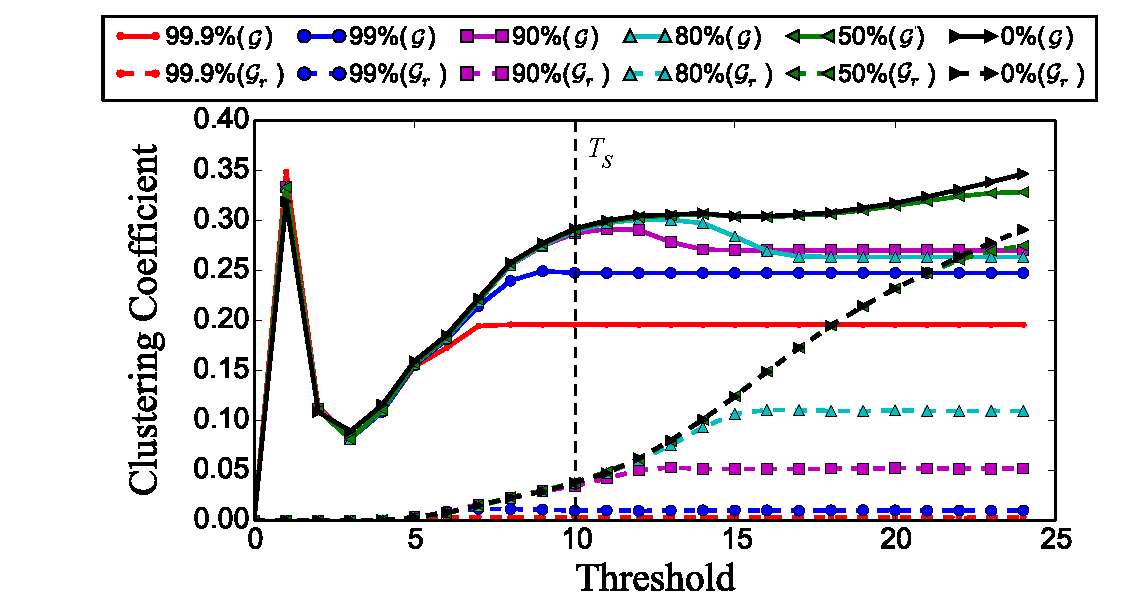
\includegraphics[width=\figSizeHundred]{ch06_patterns/figures/Characterization/CC_Curves_shrunk.pdf}
	\end{center}
	\caption{Evolution of the clustering coefficient of $\mathcal{G}$ and $\mathcal{G}_r$ over different thresholds and for different statistical confidence values used for disparity filtering (legend).}
	\label{fig:cc_curve_pattern_characterization}
\end{figure}

We next proceed to filter edges in the network based on a melodic similarity threshold $T_S$. As mentioned, determining a meaningful similarity threshold in an unsupervised setup is a challenging task. We propose to estimate $T_S$ based on the topological properties of the network. For this, we analyze the evolution of the clustering coefficient of both the obtained network $\mathcal{G}$ and the corresponding randomized network $\mathcal{G}_r$ over a range of similarity thresholds. Clustering coefficient measures the extent to which the nodes in a network tend to cluster together~\citep{newman2003structure}. The randomized network $\mathcal{G}_r$ is obtained by swapping the edges between randomly selected node pairs such that the degree of each node is preserved~\citep{maslov2002specificity}. This way, $\mathcal{G}_r$ can be considered as the maximally random network with that particular degree distribution. In~\figref{fig:cc_curve_pattern_characterization}, we show the evolution of the clustering coefficient of $\mathcal{G}$ and $\mathcal{G}_r$ over different similarity thresholds (indicated by exponentially spaced bins). In addition, we can also see the clustering coefficient curves for different statistical confidence values used for disparity filtering. The evolution of the clustering coefficients is used for obtaining a similarity threshold as explained below.

We hypothesize that the more musically meaningful $T_S$ is, the higher is the difference between the clustering coefficients of $\mathcal{G}$ and $\mathcal{G}_r$. We therefore select $T_S=10$. Note that even though the similarity threshold corresponding to $T_S=1$ results in a higher value of the clustering coefficient, we reject it because the filtered network consists only of a small number of nodes. These nodes correspond to near-exact pattern repetitions discovered within the same recording. Such patterns typically represent composition-specific motifs, and hence are irrelevant in our context. In~\figref{fig:cc_curve_pattern_characterization}, we also observe that the disparity filtering using a confidence value higher than 80\% significantly lowers the clustering coefficient, which can be attributed to the removal of musically meaningful edges in the network. On the other hand, given $T_S=10$, the disparity filtering with a confidence value lower than 80\% does not significantly affect the clustering coefficient. We can thus conclude that, in the given scenario, disparity filtering does not bring in any clear advantage. Finally, after applying $T_S$, we transform $\mathcal{G}$ to an unweighted network. 


\paragraph{Community Detection and Characterization}
\label{sec:patterns_characterization_community_detection}

We next take the unweighted undirected network that results from the previous step, and perform a non-overlapping community detection using the method proposed in~\cite{blondel2008fast}. This method is based on modularity optimization and is parameter-free from the point of view of the user. It has been extensively used in various applications~\citep{fortunato2010community} and can deal with very large networks~\citep{blondel2008fast}. We use the implementation available in networkX~\citep{hagberg-2008-exploring}, a Python language package for exploration and analysis of networks and network algorithms. Using this method for our entire dataset, we obtain around 1800 communities of melodic patterns. 


\begin{figure}
	\begin{center}
		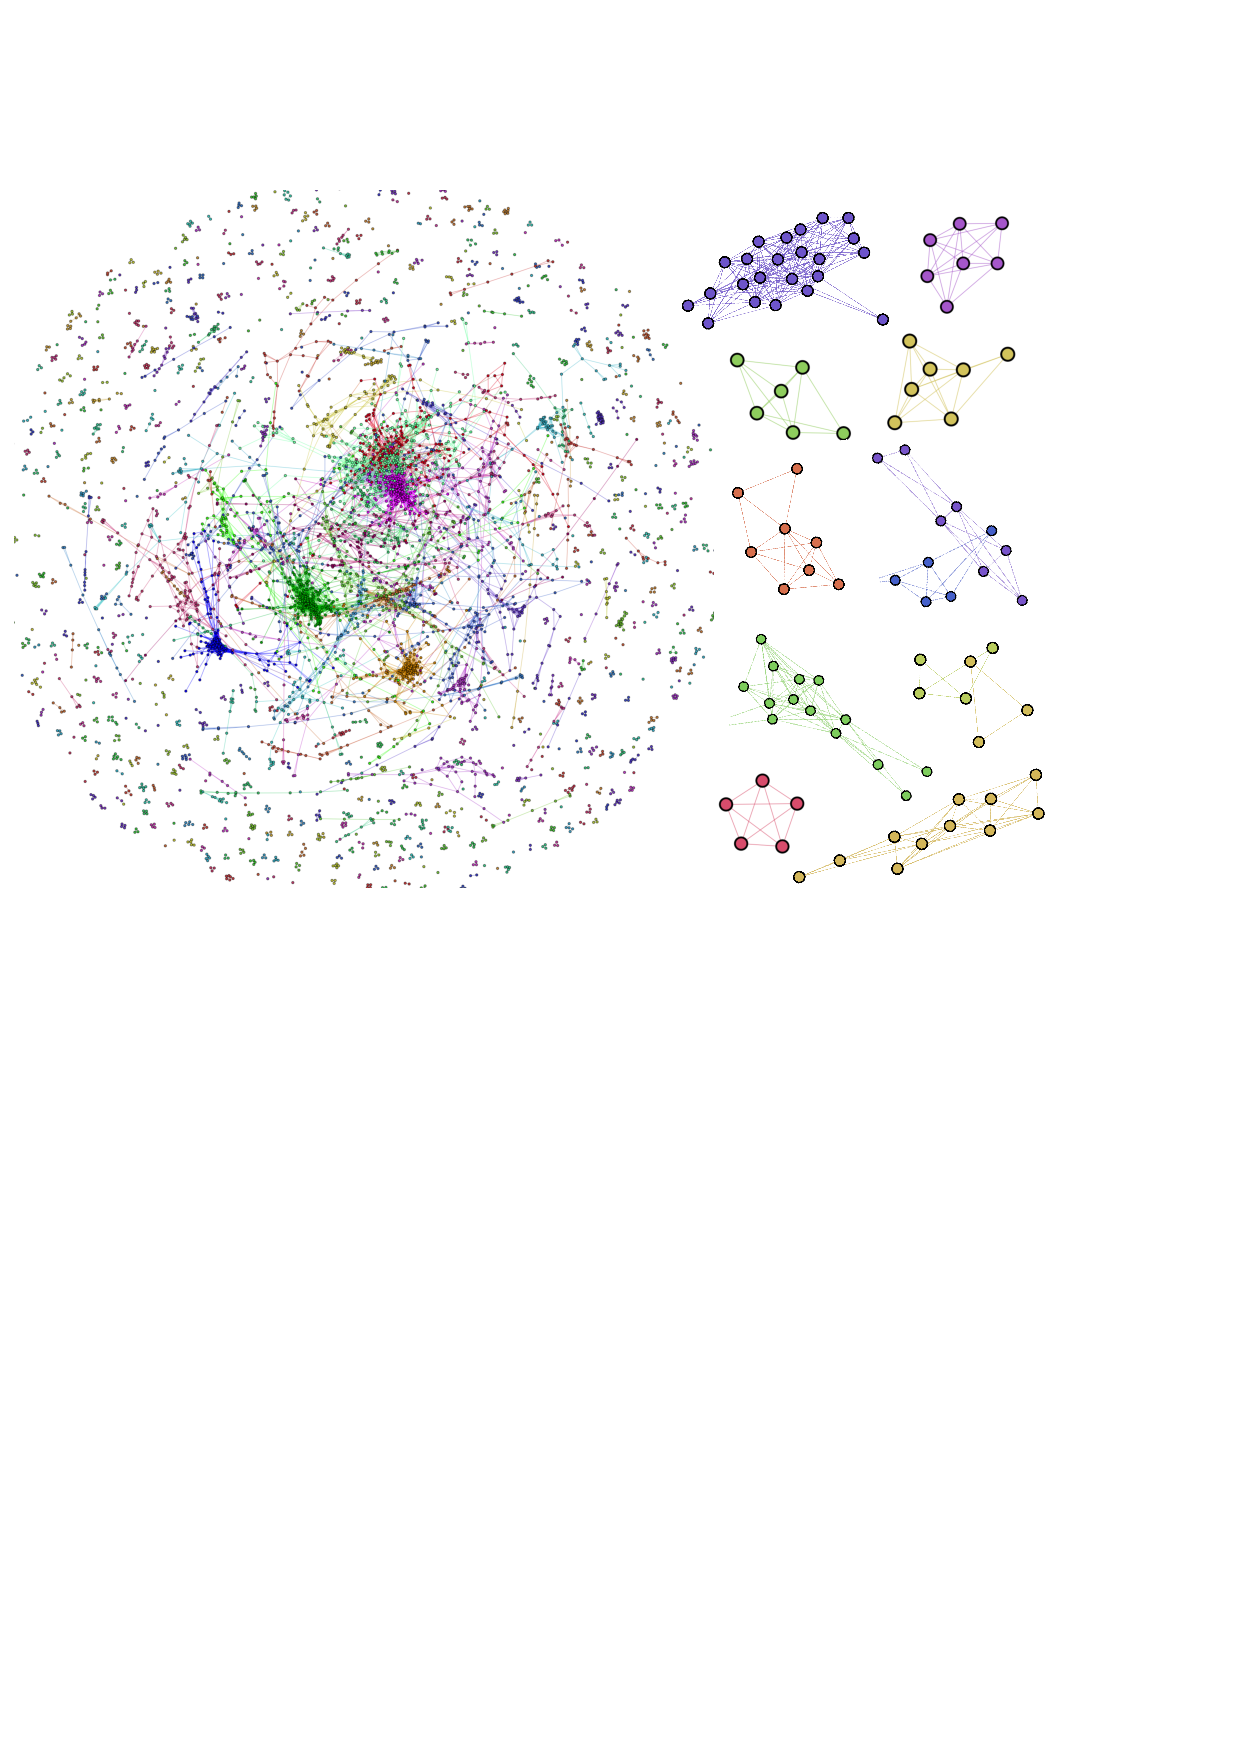
\includegraphics[width=\figSizeHundred]{ch06_patterns/figures/Characterization/networkWithClusters.pdf}
	\end{center}
 \caption{Graphical representation of the melodic pattern network after filtering by threshold $T_S$. The detected communities in the network are indicated by different colors. Few examples of these communities are shown on the right.}
 \label{fig:network_and_communities_pattern_characterization}
\end{figure}

To get a better understanding of the network obtained after filtering and the detected communities, we show a graphical representation of the network in~\figref{fig:network_and_communities_pattern_characterization}. We find that many communities comprising large number of nodes in the network correspond to Kampita melodic pattern, which is a kind of \gls{gamaka} that occur in several \glspl{raga} across compositions and hence have large number of occurrences. We also find that the communities with a relatively smaller number of nodes, which in~\figref{fig:network_and_communities_pattern_characterization} appear as isolated communities around the periphery often correspond to the \gls{raga} motifs. A few examples of such communities are shown in~\figref{fig:network_and_communities_pattern_characterization} on the right.

We here define the notation used in the subsequent paragraphs for characterizing pattern communities. A community $C_q$ is comprised of $N$ nodes, and the node count over different \glspl{raga} is given by the ordered list ${\boldsymbol{\alpha}_q} = (\alpha_{q,1}, \alpha_{q,2},\dots$ $\alpha_{q,L})$ such that $\alpha_{q,i} \geq \alpha_{q,j}$, $\forall~ i < j$,
where each element in $\alpha_{q}$ denotes the number of nodes in a particular \gls{raga} and $L$ is the total number of unique \glspl{raga} comprising the community. Similarly, the node count over the audio recordings is given by the ordered list ${\boldsymbol{\beta}_q} = (\beta_{q,1}, \beta_{q,2},\cdots,\beta_{q,K})$ such that $\beta_{q,l} \geq \beta_{q,m}, \forall~l < m$,  where each element in $\beta_{q}$ denotes the number of nodes belonging a particular audio recording and $K$ is the total number of recordings comprising the community. For both these cases, $\sum_{i=1}^{L}\alpha_{q,i} = \sum_{l=1}^{K}\beta_{q,l} = N$.

We now proceed to characterize the detected communities in order to identify the ones that represent \gls{raga} motifs. For that we first categorize a community $C_q$ as belonging to the \gls{raga} $R_q$ corresponding to the maximum number of nodes $\alpha_{q,1}$ in that community. Subsequently, for each \gls{raga}, we rank all the communities belonging to that \gls{raga}. To rank the communities we empirically devise a goodness measure $\gamma$, which denotes the likelihood that a community $C_q$ represents a \gls{raga} motif. We propose to use

\begin{equation}
\gamma = N \rho^4 \lambda,
\label{eq:gamma_pattern_characterization}
\end{equation}

where $\rho$ is an estimate of the likelihood of \gls{raga} $R_q$ in $C_q$, 

\begin{equation}
\rho = \frac{\alpha_{q,1}}{N},
\end{equation}

and $\lambda$ indicates how uniformly the nodes of the community are distributed over audio recordings,

\begin{equation}
\lambda = \frac{\sum_{l=1}^{K}l \cdot \beta_{q,l}}{N}.
\end{equation}

Higher $\lambda$ implies a more uniform distribution. Since a community that represents a \gls{raga} motif is expected to contain nodes from a single \gls{raga} (high value of $\rho$) and the nodes belong to many different recordings (high value of $\lambda$), the goodness measure $\gamma$ is high for such a community. In general we prefer large communities, but, to avoid detecting large communities (high value of N) corresponding to \gls{gamaka} motifs (low value of $\rho$) we use a fourth power on $\rho$. Composition-specific motifs are expected to have a low $\lambda$, as they are not repeated across multiple recordings, assuming that different recordings correspond to different compositions. 

Note that it might be possible that a music collection contains multiple recordings of the same composition. In such cases, differentiating composition-specific motifs and \gls{raga} motif becomes difficult using $\gamma$ measure. This issue can be overcome with only a trivial modification in our approach, i.e.,~by considering the node distribution ${\boldsymbol{\beta}_q}$ over compositions instead of recordings. In our current system this could not be implemented because for a number of recordings composition information was unavailable.



\subsection{Evaluation}
\label{sec:patterns_characterization_evaluation}

\subsubsection{Music Collection}
\label{sec:patterns_characterization_music_collection}

The music collection used in this study is a subset of the CompMusic Carnatic music corpus (\secref{sec:corpus_carnatic_music_corpus}). The collection comprises 44 hours of polyphonic audio music recordings of Carnatic music across 10 different \glspl{raga}. For each \gls{raga} we select 16 music pieces, which amounts to a total of 160 recordings. There are 139 vocal music recordings and 21 instrumental recordings comprising violin, \gls{vina} and bamboo flute. In~\tabref{tab:dataset_details_pattern_characterization}, we summarize the relevant details of the dataset. We see that it is diverse in terms of the number of unique compositions and number of lead artists. Furthermore, it includes different forms of compositions (\gls{kirtana}, varnam and viruttam) and recordings containing varied improvised sections such as \gls{alapna}, nereval and kalpan\={a}-\glspl{svara}. %The \glspl{raga} selected here are amongst the most frequently performed \glspl{raga} in the CompMusic Carnatic music corpus, which in turn is representative of the Carnatic music repertoire~\cite{CM_Corpora_Ajay14}. 
The chosen \glspl{raga} contain diverse set of \glspl{svara} (notes) both in terms of the number of \glspl{svara} and their pitch classes (svarasth\={a}n\={a}s). From~\tabref{tab:dataset_details_pattern_characterization}, 
we also notice that several \glspl{raga} such as Kaly\={a}\d{n}i, K\={a}mb\={o}ji and B\={e}gada have a large fraction of \glspl{svara} in common. We refer to them as allied \glspl{raga} (Section \TODO{XX}). This further increases the complexity of the task at hand, since the discrimination between the phrases of allied \glspl{raga} may be based on subtle melodic nuances.

\TODO{availability of the dataset?}

\begin{table} 
	%\tabcolsep = 0.1cm
	\centering
	\begin{tabular}{ l  | c c c c}
\tabletop
		\Gls{raga}   		& 	Dur 	&	\#Com		&	\#Art	&	Svaras\\	
\tablemid
		Hamsadhvani 		& 	2.46 		&	12			&	14		&	$s\,r_2\,g_3\,p\,n_3$\\
		K\={a}mavardhini 	& 	3.94 		&	13			&	16		&	$s\,r_1\,g_3\,m_2\,p\,d_1\,n_3$\\		
		Darb\={a}r   		& 	2.59 		&	8			&	13		&	$s\,r_2\,g_2\,m_1\,p\,d_2\,n_2$\\	
		Kaly\={a}\d{n}i   	& 	6.94 		&	9			&	16		&	$s\,r_2\,g_3\,m_2\,p\,d_2\,n_3$\\	
		K\={a}mb\={o}ji   	& 	6.91 		&	12			&	13		&	$s\,r_2\,g_3\,m_1\,p\,d_2\,n_2\,n_3$\\	
		B\={e}ga\d{d}a   	& 	3.41 		&	9			&	16		&	$s\,r_2\,g_3\,m_1\,p\,d_2\,n_2\,n_3$\\	
		K\={a}pi   			& 	2.24 		&	12			&	16		&	$s\,r_2\,g_2\,g_3\,m_1\,p\,d_2\,n_2\,n_3$\\	
		Bhairavi   			& 	5.33 		&	7			&	16		&	$s\,r_2\,g_2\,m_1\,p\,d_2\,d_3\,n_2$\\	
		Beh\={a}g   		& 	1.51 		&	12			&	16		&	$s\,r_2\,g_3\,m_1\,m_2\,p\,d_2\,n_2\,n_3$\\	
		
		T\={o}\d{d}i   		& 	8.75 		&	12			&	16		&	$s\,r_1\,g_2\,m_1\,p\,d_1\,n_2$\\	
\tablebot
		Total 	& 	44.08 		&	106			&	57		&	-\\	
\tablebot
	\end{tabular}
	\caption{Details of the dataset in terms of the duration (Dur) in hours, number of unique compositions (\#Com), unique lead artists (\#Art), and the svaras for each \gls{raga}. Here $s,r,$ $g,m,p,d,n$ denote the 7 svaras in IAM and the subscript indicates the variant of the svar for a particular \gls{raga} (cf.~\citep{Viswanathan2004}).}
	\label{tab:dataset_details_pattern_characterization}
\end{table}

\subsubsection{Setup and Evaluation Measures}
\label{sec:patterns_characterization_experimental_setup}

Given the unsupervised nature of this study, we perform a listening test to formally evaluate the extent to which the selected melodic phrases correspond to \gls{raga} motifs. For each of the 10 \glspl{raga} in the dataset, we select the top 10 communities based on the goodness measure $\gamma$ (\eqref{eq:gamma_pattern_characterization}). From each of these communities, we select their representative melodic phrase based on the betweenness centrality of the nodes~\citep{newman2003structure}, i.e.,~the node with the highest betweenness centrality is considered as the representative melodic phrase of that community. In case of a tie, we select the one with the highest node degree~\citep{newman2003structure}. Finally, we  arrive at a set of 100 melodic phrases, which are then used to perform the listening test. These audio examples are also made available online\footnote{http://compmusic.upf.edu/node/277}. \TODO{do we keep them at the same location?\textsl{}}

For the listening test we select 10 professional Carnatic musicians with over 15 years of formal music training. Each musician is presented with the audio fragments corresponding to the selected melodic phrases in a random order. They are also presented with the \glspl{raga} corresponding to the melodic phrases. The musicians are asked to rate each melodic phrase based on whether it is a characteristic phrase of that \gls{raga}. We use binary ratings (`Yes' or `No'). 

The audio fragments were segmented with a one second buffer on either side of the phrase to offer some context and reduce the effect of abrupt boundaries. % Thus, a 4\,s audio fragment was presented to the musicians.  
In order to quantify the musicians' assessment, we use mean ratings for each phrase $p$, $\mu_p$, considering `Yes' as 1 and `No' as 0. For analyzing the ratings per \gls{raga}, we study the mean and standard deviation of all $\mu_p$ for phrases in every \gls{raga}, which we denote by $\mu_r$ and $\sigma_r$, respectively.

\TODO{Should we say that we didn't want to not give raga since that will then bias it based on their knowledge of identifying ragas given a pattern? }

\subsection{Results and Discussion}
\label{sec:patterns_characterization_results_and_discussion}

\TODO{Is there a possibility to relate the determined similarity threshold from the one that is obtained from the discovery study, by analyzing the ROC curve???:}

We first analyze the musicians' ratings at the level of melodic phrases. In~\figref{fig:average_rating_pattern_characterization}, we show $\mu_p$ for the 100 selected melodic phrases, where the grouping is based on their corresponding \glspl{raga}. We find that the mean and the standard deviation of $\mu_p$ for the melodic phrases is 0.85 and 0.16, respectively. For a better understanding of $\mu_p$ across phrases and the overall musicians' agreement, we show the histogram of $\mu_p$ in~\figref{fig:average_rating_histogram_pattern_characterization}. We see that 33 melodic phrases are rated as \gls{raga} motifs by all 10 musicians and 25 phrases are rated as \gls{raga} motifs by 9 out of 10 musicians. Similarly, the musicians' agreement can be inferred for the rest of the phrases from this histogram. We observe that 91\% of the phrases are always marked as \gls{raga} motifs by at least 7 out of 10 musicians. 


\begin{figure}
	\begin{center}
		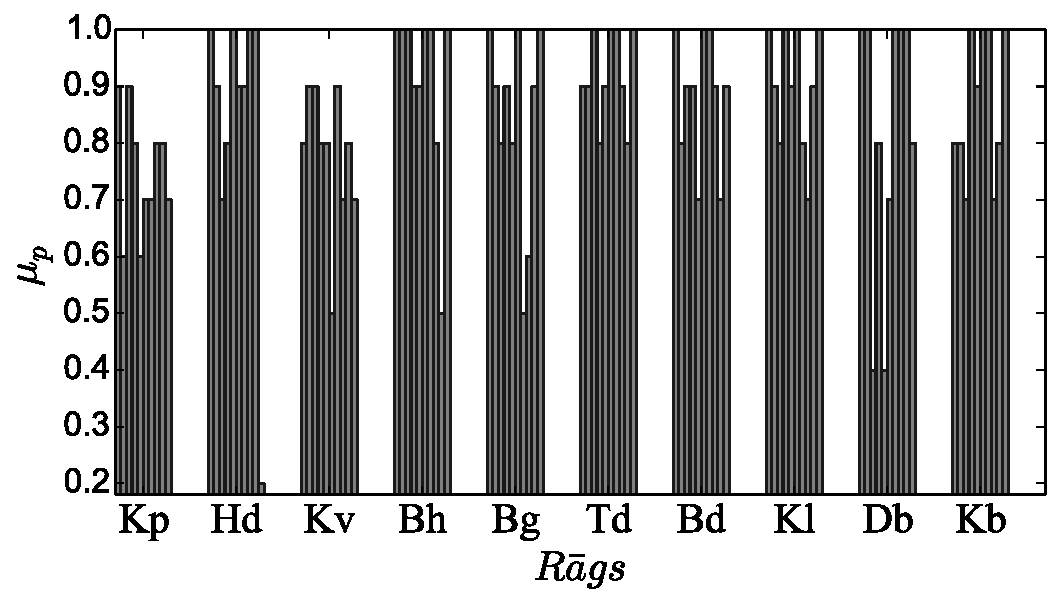
\includegraphics[width=\figSizeEighty]{ch06_patterns/figures/Characterization/per_raaga_per_phrase_rating.pdf}
	\end{center}
	\caption{Mean musician rating per melodic phrase for each \gls{raga}: K\={a}pi\,(Kp), Hamsadhvani\,(Hd), K\={a}mavardhini\,(Kv), Bhairavi\,(Bh), Beh\={a}g\,(Bg), T\={o}\d{d}i\,(Td), B\={e}ga\d{d}\={a}\,(Bd), Kaly\={a}\d{n}\={i}\,(Kl), Darb\={a}r\,(Db), K\={a}mb\={o}ji\,(Kb).}
	\label{fig:average_rating_pattern_characterization}
\end{figure}


We now proceed to analyze the results for different \glspl{raga}. In~\tabref{tab:results_per_raaga_pattern_characterization}, we summarize mean $\mu_r$ and standard deviation $\sigma_r$ of $\mu_p$ for each \gls{raga}. We observe that there is a considerable amount of variation in $\mu_r$ across the \glspl{raga}. It ranges from 0.75 for \gls{raga} K\={a}pi to 0.92 in the case of \gls{raga} T\={o}\d{d}i. An interesting observation here is that the phrase-based \glspl{raga}\footnote{R\={a}gas whose identity is derived based on phraseology than svaras~\cite{krishna2012carnatic}.\TODO{put a section ref instead of the footnote}} are the top performing \glspl{raga} with the  exception of \gls{raga} Darb\={a}r. From~\tabref{tab:results_per_raaga_pattern_characterization} and \tabref{tab:dataset_details_pattern_characterization}, we notice a strong correlation between $\mu_r$ and the total duration of the audio recordings across \glspl{raga}. This suggests that longer music pieces are likely to facilitate the discovery of \gls{raga} motifs owing to more number of occurrences of such melodic phrases.

We examine the melodic phrases with low scores. An investigation of 9 out of 100 phrases that obtain $\mu_p\leq0.6$ reveals that many of these phrases are composition-specific phrases that do not characterize the \gls{raga}. The method wrongly identifies them as \gls{raga} motifs because their associated communities have a high $\gamma$ score owing to a high $\lambda$ value. This can be attributed to the fact that these phrases are discovered from multiple recordings, since their corresponding compositions have several recordings in the dataset.  As described in~\secref{sec:patterns_characterization_community_detection}, in such a scenario, the goodness measure $\gamma$ can be made more robust to such cases by computing $\lambda$ using the distribution of nodes ${\boldsymbol{\beta}_q}$ over unique compositions rather than over audio recordings.

The results show that the proposed method successfully discovers \gls{raga} motifs with a high accuracy. We see that, even for the allied \glspl{raga} present in the dataset such as K\={a}mb\={o}ji and B\={e}gada (\secref{sec:patterns_characterization_music_collection}), the method is able to discover distinct characteristic \gls{raga} motifs. As mentioned, allied \glspl{raga} are challenging because they have a substantial overlap in the set of svaras that they comprise (see also~\tabref{tab:dataset_details_pattern_characterization}). Finally, on a more informal side, it is worth mentioning that musicians were impressed when, after the listening test, they came to know that the melodic phrases were discovered by a machine following an unsupervised approach. 


\begin{figure}
	\begin{center}
		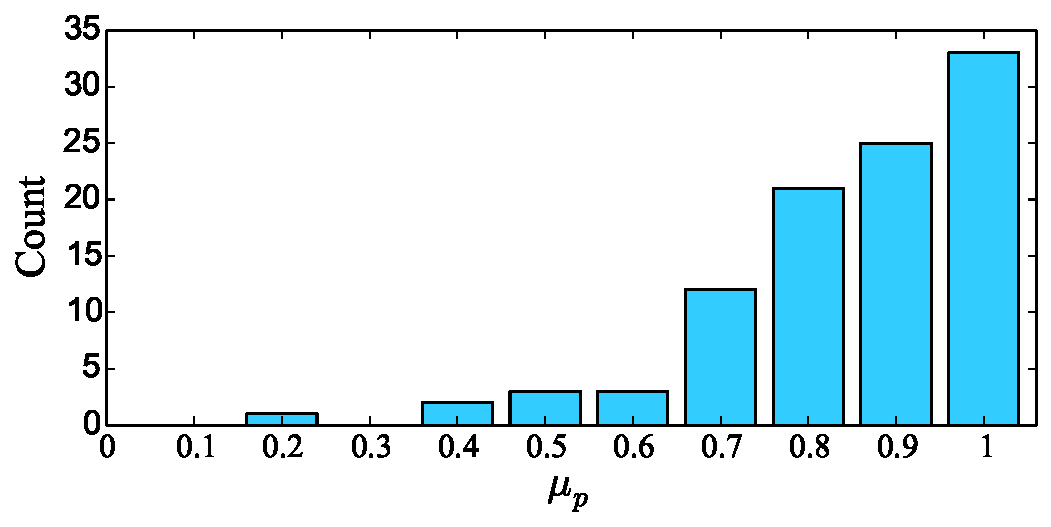
\includegraphics[width=\figSizeEighty]{ch06_patterns/figures/Characterization/histogram_musician_rating.pdf}
	\end{center}
	\caption{Histogram of $\mu_p$ for all 100 melodic phrases selected for the listening test.}
	\label{fig:average_rating_histogram_pattern_characterization}
\end{figure}


\begin{table} 
	%\tabcolsep = 0.1cm
	\centering
	\begin{tabular}{ l  c c| l | c c }
		\hline\hline
		\multicolumn{1}{ l|  }{\Gls{raga}}   			& 	$\mu_r$ 	&	$\sigma_r$	& \Gls{raga}   			& 	$\mu_r$ 	&	$\sigma_r$\\	
		\hline
		\multicolumn{1}{ l|  }{Hamsadhvani} 			& 	0.84 		&	0.23 & {\bf B\={e}ga\d{d}a}   	& 	0.88 		&	0.11	\\
		\multicolumn{1}{ l|  }{K\={a}mavardhini} 	& 	0.78 		&	0.17 & K\={a}pi   			& 	0.75 		&	0.10\\	
		\multicolumn{1}{ l|  }{Darb\={a}r}   		& 	0.81 		&	0.23 & {\bf Bhairavi}   			& 	0.91 		&	0.15\\	
		\multicolumn{1}{ l|  }{\bf Kaly\={a}\d{n}i}  & 	0.90 		&	0.10 & Beh\={a}g   		& 	0.84 		&	0.16\\	
		\multicolumn{1}{ l|  }{\bf K\={a}mb\={o}ji}   	& 	0.87 	&	0.12 & {\bf T\={o}\d{d}i}   		& 	0.92 		&	0.07\\	
		\hline\hline
		%   			& 				& 		& 	Overall&0.85 		&	0.16\\ \cline{4-6}\cline{4-6}
		%\hline\hline 
	\end{tabular}
	\caption{Mean $\mu_r$ and standard deviation $\sigma_r$ of $\mu_p$ for each \gls{raga}. R\={a}gas with $\mu_r \geq 0.85$ are highlighted. }
	\label{tab:results_per_raaga_pattern_characterization}
\end{table}


\subsection{Summary}
\label{sec:patterns_characterization_summary}

We presented a novel unsupervised approach to discover \gls{raga} motifs from polyphonic audio music collections of \gls{iam} and, specifically, to distinguish them from gamaka and composition-specific motifs. We first extracted melodic patterns from audio recordings using an unsupervised approach. We then employed a network analysis and non-overlapping community detection algorithm to cluster melodic patterns. Using the topological properties of the network, we determined a musically meaningful similarity threshold. We devised a goodness measure for characterizing the detected communities and evaluated our method using a representative music collection. A listening test with 10 professional Carnatic musicians shows that the proposed method successfully discovers \gls{raga} motifs with accuracy, even in the presence of allied \glspl{raga} in the dataset. The way we determine melodic similarity threshold and define the goodness measure appears to be successful strategies. However, only after extensive quantitative evaluations and comparisons with competing alternatives we can infer if they are the most optimal methodologies. Overall, our results suggest that the functional roles of different melodic phrases in \gls{iam} can be effectively exploited to identify them in an unsupervised manner. This, to the best of our knowledge, has been done for the first time in this study. 

\TODO{how can the results and the output of this study be utilized or helpful in other studies / applications / other use-case scenarios??}

We consider this work as a preliminary study with a lot of scope for improvements. In particular, the approach can be extended to identify patterns belonging to other categories (\gls{gamaka} or composition-specific patterns), definition of the goodness measure $\gamma$ can be improved as suggested in~\secref{sec:patterns_characterization_results_and_discussion}, listening test could be done more rigorously by including negative examples (\gls{gamaka} patterns), and the resultant patterns of the approach can be quantitatively evaluated by using them in tasks such as composition identification. On these lines, in~\secref{sec:phrase_based_feature_extraction} we present an approach that uses clustered melodic patterns to perform the task of automatic \gls{raga} recognition. That way, in addition to the qualitative assessment as done in this work, we can also quantitatively assess the musical relevance of the extracted and characterized melodic patterns.


\section{Conclusion and Future Work }
